\documentclass{article}
\usepackage{hyperref}
\usepackage{amsmath}
\usepackage{amssymb}
\usepackage{amsthm}
\usepackage{enumitem}
\usepackage{graphicx}
\usepackage{subcaption}
\usepackage{tikz}
\usepackage{tkz-graph}
\usepackage[maxnames=5]{biblatex}
\usepackage[margin=1in]{geometry}
\usepackage{mathdots}
\usepackage{dsfont}
\usetikzlibrary{shapes}

\addbibresource{quantum_csp.bib}

\newtheorem{conjecture}{Conjecture}[section]
\newtheorem{theorem}{Theorem}[section]
\newtheorem*{theorem*}{Theorem}
\newtheorem{proposition}{Proposition}[section]
\newtheorem{lemma}{Lemma}[section]
\newtheorem{corollary}{Corollary}[section]

\theoremstyle{remark}
\newtheorem{remark}{Remark}[section]
\newtheorem{claim}{Claim}[section]

\theoremstyle{definition}
\newtheorem{definition}{Definition}[section] 

\newcommand{\conjectureautorefname}{Conjecture}
\newcommand{\claimautorefname}{Claim}
\newcommand{\propositionautorefname}{Proposition}
\newcommand{\lemmaautorefname}{Lemma}
\newcommand{\definitionautorefname}{Definition}
\newcommand{\remarkautorefname}{Remark}
\newcommand{\corollaryautorefname}{Corollary}
\renewcommand{\sectionautorefname}{Section}
\renewcommand{\subsectionautorefname}{Section}

\counterwithin{figure}{section}
\counterwithin{equation}{section}

\DeclareMathOperator{\spn}{span}
\DeclareMathOperator{\tr}{tr}
\DeclareMathOperator{\rr}{\mathbb{R}}
\DeclareMathOperator{\cc}{\mathbb{C}}
\DeclareMathOperator{\arity}{arity}
\DeclareMathOperator{\vk}{\mathbf{K}}
\DeclareMathOperator{\vl}{\mathbf{L}}
\DeclareMathOperator{\vg}{\mathbf{G}}
\DeclareMathOperator{\vx}{\mathbf{x}}
\DeclareMathOperator{\vy}{\mathbf{y}}
\DeclareMathOperator{\vz}{\mathbf{z}}
\DeclareMathOperator{\va}{\mathbf{a}}
\DeclareMathOperator{\vb}{\mathbf{b}}
\DeclareMathOperator{\vq}{\mathbf{Q}}
\DeclareMathOperator{\vr}{\mathbf{R}}
\DeclareMathOperator{\vrr}{\mathbf{r}}
\DeclareMathOperator{\vc}{\mathbf{C}}
\DeclareMathOperator{\vcc}{\mathbf{c}}
\DeclareMathOperator{\vj}{\mathbf{J}}
\DeclareMathOperator{\vjj}{\mathbf{j}}
\DeclareMathOperator{\ic}{\mathcal{I}}
\DeclareMathOperator{\fc}{\mathcal{F}}
\DeclareMathOperator{\gc}{\mathcal{G}}
\DeclareMathOperator{\gk}{\mathfrak{G}_{\mathcal{F}}}
\DeclareMathOperator{\qk}{\mathfrak{Q}_{\mathcal{F}}}
\DeclareMathOperator{\ofc}{\overline{\fc}}
\DeclareMathOperator{\ogc}{\overline{\gc}}
\DeclareMathOperator{\stab}{Stab}
\newcommand{\tcwd}[1]{\left\langle #1 \right\rangle_{+, \circ, \otimes ,\top}}
\newcommand{\tcwdn}[1]{\left\langle #1 \right\rangle_{\circ, \otimes ,\top}}
\DeclareMathOperator{\holant}{Holant}
\DeclareMathOperator{\plholant}{Pl-Holant}
\DeclareMathOperator{\csp}{\#CSP}
\DeclareMathOperator{\qut}{Qut}
\DeclareMathOperator{\aut}{Aut}
\DeclareMathOperator{\eq}{\mathcal{EQ}}
\DeclareMathOperator{\geneq}{\mathcal{GEQ}}

\newcommand\numberthis{\addtocounter{equation}{1}\tag{\theequation}}
\renewcommand*{\VertexSmallMinSize}{6pt}
\newcommand{\DEdge}[2]{
    \draw[thick] (#1) -- (#2) node[draw, fill=white, kite, kite vertex angles = 120, minimum size = 4pt, inner sep = 1pt, pos=0.3, sloped] {};
}

\title{The Converse of the Real Orthogonal Holant Theorem}

\author{ Ben Young\footnote{Department of Computer Sciences, University of Wisconsin-Madison}\\
\texttt{\href{mailto:benyoung@cs.wisc.edu}{benyoung@cs.wisc.edu}}}
\date{}

\begin{document}
\maketitle

\begin{abstract}
The Holant theorem is a powerful tool for studying the computational complexity of
counting problems. Due to the great expressiveness of the Holant framework,
a converse to the Holant theorem would itself be a very powerful 
\emph{counting indistinguishability theorem}. The most general converse does not hold, but we prove
the following, still highly general, version:
if any two sets of real-valued signatures are Holant-indistinguishable, then they are equivalent 
up to an orthogonal transformation. This resolves a partially open conjecture of Xia (2010).
Consequences of this theorem include the well-known result that homomorphism counts from all graphs
determine a graph up to isomorphism, the classical sufficient condition for simultaneous orthogonal
similarity of sets of real matrices,
and a combinatorial characterization of simultaneosly orthogonally decomposable (odeco) sets of 
symmetric tensors.
\end{abstract}

\section{Introduction}
\paragraph{Holant problems.}

Holant problems were introduced by Cai, Lu, and Xia \cite{cai_computational_2011} as a highly
expressive framework for studying the computational complexity of counting problems. 
The problem $\holant(\fc)$ is defined by a set $\fc$ of \emph{signatures}, 
where a signature $F$ of \emph{arity}
$n$ on \emph{domain} $[q] := \{0,1,\ldots,q-1\}$ is a tensor in $(\cc^q)^{\otimes n}$. 
Given a \emph{signature grid} $\Omega$ -- a multigraph in which every degree-$n$ vertex is assigned a
$n$-ary signature from $\fc$ --
the problem is to compute the \emph{Holant value} of $\Omega$, which is the value
of the contraction of $\Omega$ as a tensor network (see \autoref{sec:holant} for formal definitions). 
For various $\fc$, $\holant(\fc)$ captures a wide variety of natural counting problems on
graphs, including counting partial or perfect matchings, graph homomorphisms, 
proper vertex or edge-colorings, or Eulerian orientations.
Major complexity dichotomies classifying $\holant(\fc)$ as either 
polynomial-time tractable or \#P-hard,
depending on $\fc$, have been proved for various combinations of restrictions on $\fc$ -- for example,
requiring that the signatures in $\fc$ be real- or nonnegative-real-valued, symmetric
(invariant under reordering of their inputs), or on the Boolean domain $q=2$
\cite{huang_2016_dichotomy,cai_complete_2016,cai2015holant,lin_complexity_2018,shao}.

Holant problems were motivated by Valiant's technique of \emph{holographic
transformations} \cite{valiant}. In particular, Valiant's \emph{Holant theorem} (\autoref{thm:holant}
below) states roughly that two any signature sets $\fc \cup \fc'$ and $\gc \cup \gc'$ that are 
equivalent up to a certain 
linear transformation are \emph{Holant-indistinguishable}, meaning that each signature grid $\Omega$
has the same Holant value whether its vertices are assigned signatures from $\fc \cup \fc'$ or from 
$\gc \cup \gc'$.
Many problems which do not otherwise appear tractable are in fact tractable under a Holographic
transformation to a known tractable problem \cite{valiant_2006_accidental}.
Xia \cite{xia} conjectured the converse of the Holant theorem: if $\fc \cup \fc'$ and
$\gc \cup \gc'$ are Holant-indistinguishable, then they are equivalent up to linear transformation.
Xia's general conjecture is false (see \autoref{sec:holanttheorem}), but one case highlighted
by Xia was left open. This paper proves that case, which is as follows.
\begin{theorem*}[\autoref{thm:result}, informal]
    Let $\fc$ and $\gc$ be sets of real-valued signatures. Then $\fc$ and $\gc$ are equivalent under
    a real orthogonal transformation if and only if $\fc$ and $\gc$ are Holant-indistinguishable.
\end{theorem*}

\paragraph{Vertex and edge coloring models.}
This work uses and generalizes ideas from the theory of vertex coloring models and edge coloring models,
two well-studied classes of Holant problems.
De la Harpe and Jones \cite{jones} defined vertex and edge coloring models as extensions of 
statistical mechanics models (e.g. the Ising model), calling them ``spin models'' and ``vertex models'',
respectively. A vertex coloring model is defined by a graph $X$ with edge and possibly vertex
weights. Given an input graph $K$, one aims to compute the \emph{partition function}, the number of 
(weighted) homomorphisms from $K$ to $X$.
As discussed in \autoref{sec:holant}, computing the partition function of a vertex coloring model
without vertex weights is equivalent to $\holant(A_X \cup \eq)$, where
$A_X$ is the weighted adjacency matrix of $X$ and $\eq$ is the set of \emph{equality} signatures 
(we can model vertex weights by replacing $\eq$ with $\geneq$, the set of weighted equalities).
An edge coloring model is defined by a set $\fc$ of symmetric signatures containing exactly
one signature of each arity, and the problem of computing its partition function is equivalent to 
$\holant(\fc)$ (this restriction on $\fc$ ensures that
edge coloring models take ordinary graphs, rather than signature grids, as input).

One thread of prior work on vertex and edge coloring models 
characterizes which graph parameters (scalar-valued functions defined on isomorphism classes of graphs)
are expressible as vertex coloring models \cite{freedman_reflection, schrijver}
or as edge coloring models 
\cite{szegedy_edge_2007, schrijver_graph_2008, draisma_characterizing_2012, regts_characterization_2013}.
Another, related, line of works compute the rank of \emph{connection matrices}
for vertex coloring models \cite{lovasz} and edge coloring models 
\cite{regts_rank_2012,draisma_tensor_2013}.
See Regts' thesis \cite{regts} for an overview of many of the above results. 
Following Freedman, Lov\'{a}sz, and Schrijver \cite{freedman_reflection}, these works all use
some form of (labeled) \emph{quantum graphs}, algebras of formal linear combinations of graphs 
equipped with labeled vertices or ``half edges'' incident to a single vertex. Each labeled quantum
graph defines a tensor by evaluating its partition function when its labeled vertices
are fixed to input values. All such constructions are special cases of our 
\emph{quantum gadgets} below (see \autoref{def:quantum_gadget}).
Many of these works also apply techniques from invariant theory, either of the symmetric group
in the case of vertex coloring models \cite{schrijver}, or, as in this work, of the
orthogonal group $O(q)$ in the case of edge-coloring models \cite{szegedy_edge_2007, schrijver_graph_2008, draisma_characterizing_2012, regts_rank_2012, draisma_tensor_2013, regts_characterization_2013}.

\paragraph{Counting Indistinguishability Theorems.}
\autoref{thm:result} is a very general and powerful algebraic 
\emph{counting indistinguishability theorem}. 
Such a theorem proves that two signatures, or sets of signatures, are indistinguishable
as parameters for a counting problem if and only if they are equivalent under an algebraic
transformation. These theorems exist for both vertex and edge coloring models, as well as other
counting problems \cite{dell, grohe_homomorphism_2022, dvorak_recognizing_2010}.
Since the Holant framework captures a wide variety of counting problems,
including both vertex and edge coloring models, many such theorems are special cases
of \autoref{thm:result} (see \autoref{sec:corollaries}).
If the counting problem in question is a generalized vertex coloring model ($\holant(\fc \cup \eq)$
for some $\fc$), then the algebraic transformation is isomorphism, and if the counting problem is,
as in this work, a generalized edge coloring model, then it is orthogonal.
The first counting indistinguishability theorem, proved by Lov\'{a}sz \cite{lovasz_operations}, 
states that two graphs are
isomorphic if and only if they admit the same number of homomorphisms from all graphs. Much later,
Lov\'{a}sz \cite{lovasz} extended this theorem to vertex coloring models with nonnegative real 
weights, followed by extensions to complex edge weights by Schrijver 
\cite{schrijver}, and to weights from any field of characteristic zero by Cai and Govorov 
\cite{cai-lovasz}. Young \cite{young2022equality} extended Cai and Govorov's proof to \#CSP, or
$\holant(\fc \cup \eq)$ for any $\fc$. 

For edge coloring models, Schrijver \cite{schrijver_graph_2008} showed that 
$\fc$ and $\gc$ define indistinguishable real edge coloring models if and only if
$\fc$ and $\gc$ are equivalent under a real orthogonal transformation. 
This is a special case of our \autoref{thm:result}.
Schrijver's proof exploits the specific nature of edge coloring models -- that $\fc$ and $\gc$ consist
of symmetric signatures and exactly one signature per arity -- to transform input graphs into polynomials
expressible in variables $y_1,\ldots,y_q$ (for $\fc$ and $\gc$ on domain $[q]$), 
where a monomial with variable multiset $\{y_{i_1},\ldots, y_{i_n}\}$ corresponds to the
$\{i_1,\ldots,i_n\}$-entry of the unique $n$-ary signature in $\fc$.
Another form of this result (in which the orthogonal matrix is allowed to be complex) 
follows from Regts' proof of 
\cite[Lemma 5]{regts_characterization_2013}, which similarly encodes $\fc$ and $\gc$ as polynomials.

Man\v{c}inska and Roberson \cite{planar} introduced a new form of counting indistinguishability
theorem, showing that two graphs are \emph{quantum isomorphic} -- an abstract relaxation of isomorphism
-- if and only if they admit the same number of homomorphisms from all planar graphs.
Cai and Young \cite{cai_planar_2023} translated Man\v{c}inska and Roberson's proof into the Holant 
framework (we adopt many of Cai and Young's definitions and notations in this paper) and extended it to 
planar $\csp$ (or $\plholant(\fc \cup \eq)$, where $\plholant$ restricts to planar signature grids), showing that real-valued $\fc$ and $\gc$ are planar-$\csp$-indistinguishable if and
only if they are quantum isomorphic.

\paragraph{Odeco signature sets}
A real-valued symmetric signature (tensor) is \emph{orthogonally decomposable}, 
or \emph{odeco} \cite{robeva}, if it is orthogonally transformable to a signature in $\geneq$, the set
of \emph{generalized equality} signatures, which take nonzero values only when all of their inputs
are equal. Hence odeco tensors generalize diagonalizable matrices.
Call a set $\fc$ of signatures odeco if the signatures are simultaneously odeco (there
is a single orthogonal transformation mapping $\fc$ into $\geneq$).
In counting complexity, if $\fc$ is odeco, then
$\holant(\fc)$ is polynomial-time tractable, as $\fc$ maps into $\geneq$, a trivially tractable set,
under an orthogonal holographic transformation.
Indeed, the tractability of \emph{Fibonacci} signature sets \cite{cai2008holographic}
can, with one exception, be explained by such 
sets being simultaneously odeco (see e.g. \cite[Section 2.2]{cai_chen_2017}). 
Fibonacci sets constitute almost all nontrivial tractable cases of $\holant^*$ problems
(an important variant of Holant in which all unary signatures are assumed 
present) for symmetric signatures on the Boolean domain \cite{cai_computational_2011}.
Simultaneously odeco
sets provide a natural starting point for extending Fibonacci signatures to higher
domains \cite{liu_2024}, where no full complexity dichotomy for $\holant^*$ is known.

Boralevi, Draisma, Horobeţ, and Robeva \cite{boralevi_orthogonal_2017}, resolving a conjecture of
Robeva \cite{robeva}, showed using techniques from algebraic geometry that a single tensor $F$ is 
odeco if and only if the signature of 
a certain $F$-gadget is symmetric. Using \autoref{thm:result}, we in \autoref{thm:odeco} extend this 
characterization to sets of simultaneously odeco signatures: $\fc$ is odeco if and only if every connected 
$\fc$-gadget has a symmetric signature. This deepens the connection between Fibonacci and odeco 
signatures, as the original proof of tractability of any Fibonacci signature set $\fc$
\cite{cai2008holographic} relied on the fact that every connected $\fc$-gadget has a signature which is
itself Fibonacci (in particular, is symmetric). 
One can view the (iii) $\implies$ (ii) result in \autoref{thm:odeco} as a general-domain version
of this proof.

\paragraph{Overview.}
We introduce the necessary preliminaries and formally state \autoref{thm:result} in 
\autoref{sec:preliminaries}. 
In \autoref{sec:duality}, we use an invariant-theoretic
result of Schrijver \cite{schrijver_tensor_2008} (\autoref{thm:duality}) to prove a
combinatorial-algebraic duality (\autoref{thm:intertwiner_gadget}) showing that
combinatorial quantum $\fc$-gadgets exactly capture all tensors invariant under the algebraic
action of $\stab(\fc)$, the group of orthogonal transformations stabilizing $\fc$.
The proof of \autoref{thm:intertwiner_gadget} entails characterizing quantum $\fc$-gadgets as the
algebra generated by a few fundamental gadgets under operations which respect the action of
$O(q)$. It follows and generalizes a proof of a similar result of Regts \cite{regts_rank_2012}
for edge coloring models. By unifying the perspective of Regts with that of
Man\v{c}inska and Roberson and Cai and Young \cite{planar, cai_planar_2023, young2022equality} we find
that our proof is also strongly analogous to proofs of similar results in the latter line of work
(see \autoref{rem:duality}). 

However, Man\v{c}inska and Roberson and Cai and Young's proofs of their ensuing
counting indistinguishability theorems use the \emph{orbits} and/or
\emph{orbitals} of the action of the symmetric or quantum symmetric group on the domain set $[q]$,
which do not exist for $O(q)$. Instead, we apply a novel method: induction on the domain
size $q$. We show in \autoref{lem:induction} that, if $\fc$ and $\gc$ contain a binary signature
represented by a nontrivial (i.e., not a multiple of $I$) diagonal matrix, then we can separate $[q]$
into smaller subdomains and apply induction to obtain successive orthogonal transformations between 
the restrictions of $\fc$ and $\gc$ to each subdomain, producing a full orthogonal transformation from 
$\fc$ to $\gc$. Using \autoref{thm:intertwiner_gadget},
we show that there is some nonzero matrix $D$ intertwining $\fc$
and $\gc$. Exploiting the power of diagonalization afforded by orthogonal transformations, we may
assume this $D$ is diagonal. Either $D = \pm I$, giving a trivial orthogonal transformation between
$\fc$ and $\gc$, or $D$ is not a multiple of $I$, in which case we use the fact that $D$ intertwines
$\fc$ and $\gc$ to add $D$ to both $\fc$ and $\gc$ while preserving their Holant-indistinguishability, 
then apply induction.

In \autoref{sec:corollaries}, we show that \autoref{thm:result} 
encompasses a wide range of existing counting indistinguishability theorems,
and yields some novel variations of these theorems. We also prove our combinatiorial characterization of
odeco signature sets.

Finally, in \autoref{sec:variations}, we discuss two possible variations of \autoref{thm:result}.
First for complex-valued signatures, and second for an extension of the results 
of Man\v{c}inska and Roberson \cite{planar} and Cai and Young \cite{cai_planar_2023} 
to planar-Holant-indistinguishability and quantum orthogonal transformations.
 \section{Preliminaries, Background, and the Main Theorem}
\label{sec:preliminaries}
\subsection{Holant Problems}
\label{sec:holant}
Let $\mathbb{N}$ be the set of natural numbers, including 0.
A \emph{signature} $F$ of finite \emph{arity} $n \in \mathbb{N}$ on finite \emph{domain} $V(F)$ is function $V(F)^n \to \rr$.
We will often take $V(F) = [q] := \{0,1,\ldots,q-1\}$, in which case we also view $F$ as a
tensor in $(\rr^q)^{\otimes n}$. For $\vx = (x_1,\ldots,x_n) \in V(F)^n$, abbreviate
$F_{\vx} := F(x_1,\ldots,x_n) \in \rr$. Signature $F$ is \emph{symmetric} if 
its value depends only on the multiset of inputs, not on their order.
Any time we consider a set $\fc$ of signatures,
we assume that all signatures in $\fc$ have the same domain, denoted $V(\fc)$. 

In the context of a signature set $\fc$, a
\emph{signature grid} (or \emph{$\fc$-grid}) $\Omega$ consists of an underlying multigraph with 
vertex set $V$ and edge set $E$, and an assignment of an $\deg(v)$-ary signature $F_v \in \fc$ 
to each $v \in V$, along with an ordering of the edges $\delta(v) \subset E$ incident to $v$ 
to serve as the
$\deg(v)$ input variables to $F$. That is, there is an ordering $e_1,\ldots,e_{\deg(v)}$ of $v$'s 
incident edges such that, if $\sigma: E \to V(\fc)$ is an assignment of a value in $V(\fc)$ to each
edge of $\Omega$, then $F_v$ evaluates to 
$F_v(\sigma|_{\delta(v)}) := F_v(\sigma(e_1),\ldots,\sigma(e_{\deg(v)}))$.
Somewhat unusually, we also allow $E$ to contain \emph{vertexless loops}, edges whose two ends are 
connected to each other, with no incident vertices.
The problem $\holant(\fc)$ is defined as follows: given an $\fc$-grid $\Omega$
with vertex set $V$ and edge set $E$, compute the \emph{Holant value}
\begin{equation}
    \holant_\Omega(\fc) := \sum_{\sigma: E \to V(\fc)} \prod_{v \in V} F_v(\sigma|_{\delta(v)}).
    \label{eq:holant}
\end{equation}
When $\fc$ is clear from context, we abbreviate $\holant_\Omega(\fc)$ as 
$\holant_\Omega$. Each vertexless loop of $\Omega$ contributes a global factor $|V(\fc)|$ to
$\holant_\Omega$. More generally, the Holant value of a disconnected signature grid
is the product of the Holant values of its connected components.
For signature sets $\fc$ and $\fc'$, define $\holant(\fc \mid \fc')$ as the Holant problem 
whose input is a bipartite $(\fc\sqcup\fc')$-grid 
$\Omega$, with the vertices in the two bipartitions assigned signatures in $\fc$ and $\fc'$,
respectively.

For example, if $\fc$ is on the Boolean domain $\{0,1\}$ and consists of, for each arity $n$, a symmetric
signature which evaluates to 1 on input strings of Hamming weight 1 and 0 on all other input strings,
then $\holant_{\Omega}(\fc)$ equals the number of perfect matchings in the multigraph underlying
$\Omega$. For another example, let $A_X \in \rr^{q \times q}$ be the 
adjacency matrix of $q$-vertex weighted graph $X$, and define the set
$\eq = \{=_n \mid n \geq 1\}$ of \emph{equality}
signatures, where $=_n(x_1,\ldots,x_n)$ is 1 if $x_1 = \ldots = x_n$, and is 0 otherwise. 
Consider $\holant(A_X \mid \eq)$. We can think of any edge assignment
$\sigma$ with a nonzero contribution to the Holant value as a map from vertices in $\Omega$ assigned
$\eq$ signatures to values in $[q]$, or equivalently vertices of $X$. This map must send the two 
$\eq$ vertices
adjacent to every $A_X$ vertex to an edge in $A_X$, so, if $K$ is the graph resulting from ignoring
(i.e. treating as edges) the degree-two vertices assigned $A_X$ in the underlying graph of $\Omega$,
then $\holant_{\Omega}(A_X \mid \eq)$ equals the number of graph homomorphisms from $K$ to $X$.
See \autoref{fig:hom}.
\begin{figure}[ht!]
    \centering
    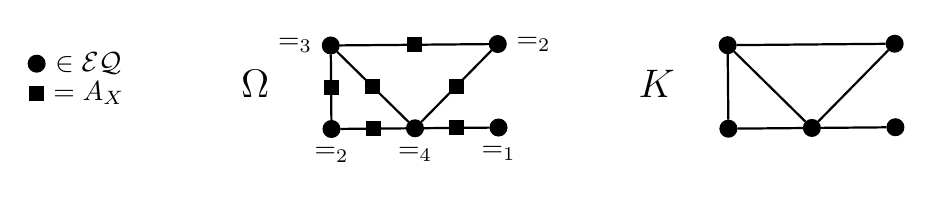
\begin{tikzpicture}[scale=0.75]
    \GraphInit[vstyle=Classic]
    \SetUpEdge[style=-]
    \SetVertexMath

    \def\xshift{6}


    \begin{scope}[rotate=-44.5]
        \Vertex[x=0,y=1,NoLabel]{a1}
        \Vertex[x=2,y=3,NoLabel]{b1}
        \Vertex[x=2,y=1,NoLabel]{c1}
        \Vertex[x=1,y=0,NoLabel]{d1}
        \Vertex[x=3,y=2,NoLabel]{e1}
    \end{scope}

    \begin{scope}[xshift=-11cm, yshift=4.2cm, rotate=-44.5]
\Vertex[x=0+\xshift,y=1,L={=_3},Lpos=180]{a2}
        \Vertex[x=2+\xshift,y=3,L={=_2},Lpos=0]{b2}
        \Vertex[x=2+\xshift,y=1,L={=_4},Lpos=270]{c2}
        \Vertex[x=1+\xshift,y=0,L={=_2},Lpos=270]{d2}
        \Vertex[x=3+\xshift,y=2,L={=_1},Lpos=270]{e2}


\tikzset{VertexStyle/.style = {shape=rectangle, fill=black, minimum size=5pt, inner sep=1pt, draw}}
        \Vertex[x=1+\xshift,y=2,NoLabel]{ax1}
        \Vertex[x=1+\xshift,y=1,NoLabel]{ax2}
        \Vertex[x=0.5+\xshift,y=0.5,NoLabel]{ax3}
        \Vertex[x=1.5+\xshift,y=0.5,NoLabel]{ax4}
        \Vertex[x=2+\xshift,y=2,NoLabel]{ax5}
        \Vertex[x=2.5+\xshift,y=1.5,NoLabel]{ax6}

    \end{scope}

    \foreach \xs/\num in {0/1,\xshift/2} {
        \Edges(a\num,b\num,c\num,d\num,a\num,c\num,e\num)
    };

    \node[font=\Large] at (-7.3,0.05) {$\Omega$};
    \node[font=\Large] at (-0.5,0.05) {$K$};

\Vertex[x=-11,y=0.4,L={\in \eq}]{ax8}
    \tikzset{VertexStyle/.style = {shape=rectangle, fill=black, minimum size=5pt, inner sep=1pt, draw}}
    \Vertex[x=-11,y=-0.1,L={=A_X}]{ax7}

\end{tikzpicture}
     \caption{An $(A_X \mid \eq)$-grid $\Omega$ and the graph $K$ such that $\holant_\Omega(A_X \mid \eq)$
    counts the number of homomorphisms from $K$ to $X$.}
    \label{fig:hom}
\end{figure}

\subsection{Gadgets and Signature Matrices}
Instead of viewing a signature $F$ as a tensor in $(\rr^q)^{\otimes n}$ or function in $\rr^{[q]^n}$,
we can partition its inputs in two to view it naturally as a matrix.
\begin{definition}[$F^{m,d},f$]
    \label{def:sig_matrix}
    For $F \in (\rr^q)^{\otimes n}$ and $m,d \in \mathbb{N}$ with $m+d=n$, define the 
    $(m,d)$-\emph{signature matrix}, or \emph{flattening}, $F^{m,d} \in \rr^{q^m\times q^d}$ of $F$
    by, for $\vx \in [q]^m$ and $\vy \in [q]^d$,
    \[
        (F^{m,d})_{\vx,\vy} = F(x_0,\ldots,x_{m-1},y_{d-1},\ldots,y_0),
    \]
    where we use the standard isomorphism $[q^n] \cong [q]^n$ to index $F^{m,d}$.

    Abbreviate $f = F^{n,0} \in \rr^{q^n}$ -- the (column) \emph{signature vector} of $F$.
\end{definition}
We will often identify binary signatures in $(\rr^q)^{\otimes 2}$
with their $1,1$ signature matrices in $\rr^{q \times q}$.
\begin{definition}[$\gk,\gk(m,d)$]
    For signature set $\fc$, an $\fc$-\emph{gadget} is a $\fc$-grid equipped with an ordered set of
    \emph{dangling edges} with zero or one endpoints.

    Define $\gk$ to be the set of all $\fc$-gadgets, and $\gk(m,d) \subset \gk$ to be the set of gadgets
    with $m+d$ dangling edges $\ell_0, \ldots, \ell_{m-1}, r_{d-1}, \ldots, r_0$ drawn with dangling
    ends in counterclockwise cyclic order around the gadget, with
    $\ell_0, \ldots, \ell_{m-1}$ and $r_{0}, \ldots, r_{d-1}$ on the left 
    and right, respectively, from top to bottom.
\end{definition}
See \autoref{fig:gadgetops} for examples of gadgets.
A gadget in $\gk(m,d)$ defines a $(m+d)$-ary signature in flattened form, with dangling edges representing
inputs, as follows (cf. \eqref{eq:holant}):
\begin{definition}[$M(\vk)$]
    \label{def:gadget_sig_matrix}
    Define the \emph{signature matrix} $M(\vk) \in \rr^{q^m \times q^d}$ of $\vk \in \gk(m,d)$ by
    \[
        M(\vk)_{\vx,\vy} = \sum_{\substack{\sigma: E(\vk) \to [q] \\ \forall i: \sigma(\ell_i) = x_i 
        \\ \forall j: \sigma(r_j) = y_{j}}}\prod_{v \in V} F_v(\sigma|_{\delta(v)})
        ~~\text{ for $\vx \in [q]^m$ and $\vy \in [q]^d$}.
    \]
\end{definition}
If $\vk \in \gk(m,d)$ is a gadget consisting
of a single vertex assigned $F$ with $m$ and $d$ incident left and right dangling edges, 
respectively, ordered to match the input order of $F$, then $M(\vk) = F^{m,d}$.
In general, for $\vk \in \gk(m,d)$, there is a unique $F \in (\rr^q)^{\otimes m+d}$, called the \emph{signature of} $\vk$,
such that $M(\vk) = F^{m,d}$. Note that $F$ does not depend on the
particular left/right partition (i.e. choice of $m$ and $d$) of a fixed cyclic order 
of $\vk$'s dangling edges.
\begin{definition}[$\circ, \otimes, \top$]
    Define the following three operations on gadgets:
    \begin{itemize}
        \item For $\vk \in \gk(m,d)$ and $\vl \in \gk(d,r)$, construct $\vk \circ \vl \in \gk(m,r)$
            by connecting the dangling ends of $r_i \in E(\vk)$ and $\ell_i \in E(\vl)$ for $i \in [d]$.
        \item For $\vk \in \gk(m_1,d_1)$ and $\vl \in \gk(m_2,d_2)$, construct 
            $\vk \otimes \vl \in \gk(m_1+m_2,d_1+d_2)$ as the disjoint union of $\vk$ and $\vl$,
            placing $\vk$ above $\vl$. Interleave $\vk$ and $\vl$'s dangling edges into
            an overall cyclic order: $\vk$ left, then $\vl$ left, then $\vl$ right, then $\vk$ right.
        \item For $\vk \in \gk(m,d)$, construct $\vk^{\top} \in \gk(d,m)$ 
            by exchanging the roles of left and right dangling edges and reversing
            the overall cyclic dangling edge order (visually, horizontally reflect $\vk$).
    \end{itemize}
\end{definition}
See \autoref{fig:gadgetops}. As one might expect,
the gadget operations $\circ, \otimes, \top$ induce the respective operations -- composition, 
Kronecker product, transpose -- on their signature matrices. See e.g. 
\cite[Section 1.3]{cai_chen_2017}.
\begin{figure}[ht!]
    \begin{center}
    \begin{subfigure}{0.8\textwidth}
        \centering
        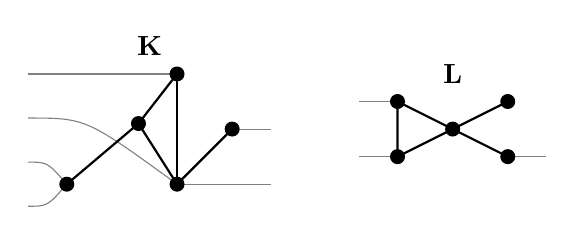
\begin{tikzpicture}[scale=0.7]
    \GraphInit[vstyle=Classic]
    \SetUpEdge[style=-]
    \SetVertexMath
    \tikzset{VertexStyle/.style = {shape=circle, fill=black, minimum size=5pt, inner sep=1pt, draw}}

\def\wirelen{0.7}
    \def\xsh{7}

\draw[thin, color=gray] (-\wirelen,-0.4) .. controls (-\wirelen/2,-0.4) .. (0,0);
    \draw[thin, color=gray] (-\wirelen,0.4) .. controls (-\wirelen/2,0.4) .. (0,0);
    \draw[thin, color=gray] (-\wirelen,2) -- (2,2);
    \draw[thin, color=gray] (2,0) -- (3+\wirelen,0);
    \draw[thin, color=gray] (3,1) -- (3+\wirelen,1);
    \draw[thin, color=gray] (-\wirelen,1.2) .. controls (\wirelen/2,1.2) .. (2,0);

    \Vertex[x=1.3,y=1.1,NoLabel]{ax1}
    \Vertex[x=0,y=0,NoLabel]{a2}
    \Vertex[x=2,y=2,NoLabel]{b2}
    \Vertex[x=2,y=0,NoLabel]{c2}
    \Vertex[x=3,y=1,NoLabel]{e2}

    \Edges(a2,ax1,b2,c2)
    \Edges(c2,e2)


    \Edge(c2)(ax1)

    \node at (1.5,2.5) {$\mathbf{K}$};

\def\ysh{0.5}
    \draw[thin, color=gray] (\xsh+1+\wirelen,0+\ysh) -- (\xsh+1,0+\ysh);
    \draw[thin, color=gray] (\xsh+-1,0+\ysh) -- (\xsh-1-\wirelen,0+\ysh);
    \draw[thin, color=gray] (\xsh+-1,1+\ysh) -- (\xsh-1-\wirelen,1+\ysh);

    \tikzset{VertexStyle/.style = {shape=circle, fill=black, minimum size=5pt, inner sep=1pt, draw}}
    \Vertex[x=\xsh+1,y=0+\ysh,NoLabel]{a3}
    \Vertex[x=\xsh+1,y=1+\ysh,NoLabel]{b3}
    \Vertex[x=\xsh-1,y=0+\ysh,NoLabel]{c3}
    \Vertex[x=\xsh-1,y=1+\ysh,NoLabel]{e3}

    \node at (\xsh, 1.5+\ysh) {$\mathbf{L}$};

    \Vertex[x=\xsh+0,y=0.5+\ysh,NoLabel]{bx3}

    \Edges(e3,c3,b3)
    \Edge(e3)(a3)
\end{tikzpicture}
     \end{subfigure}

    \begin{subfigure}{0.4\textwidth}
        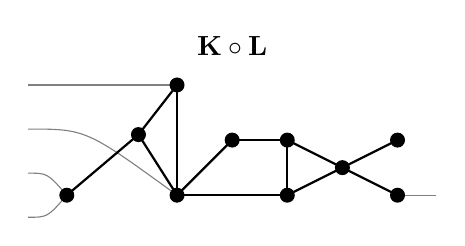
\begin{tikzpicture}[scale=0.7]
    \GraphInit[vstyle=Classic]
    \SetUpEdge[style=-]
    \SetVertexMath
    \tikzset{VertexStyle/.style = {shape=circle, fill=black, minimum size=5pt, inner sep=1pt, draw}}

\def\wirelen{0.7}
    \def\xsh{5}

    \node at (\xsh-2, 2.7) {$\mathbf{K} \circ \mathbf{L}$};

\draw[thin, color=gray] (-\wirelen,-0.4) .. controls (-\wirelen/2,-0.4) .. (0,0);
    \draw[thin, color=gray] (-\wirelen,0.4) .. controls (-\wirelen/2,0.4) .. (0,0);
    \draw[thin, color=gray] (-\wirelen,2) -- (2,2);
    \draw[thin, color=gray] (-\wirelen,1.2) .. controls (\wirelen/2,1.2) .. (2,0);

    \Vertex[x=1.3,y=1.1,NoLabel]{ax1}
    \Vertex[x=0,y=0,NoLabel]{a2}
    \Vertex[x=2,y=2,NoLabel]{b2}
    \Vertex[x=2,y=0,NoLabel]{c2}
    \Vertex[x=3,y=1,NoLabel]{e2}

    \Edges(a2,ax1,b2,c2)
    \Edge(c2)(ax1)
    \Edge(c2)(e2)

\draw[thin, color=gray] (\xsh+1+\wirelen,0) -- (\xsh+1,0);

    \tikzset{VertexStyle/.style = {shape=circle, fill=black, minimum size=5pt, inner sep=1pt, draw}}
    \Vertex[x=\xsh+1,y=0,NoLabel]{a3}
    \Vertex[x=\xsh+1,y=1,NoLabel]{b3}
    \Vertex[x=\xsh-1,y=0,NoLabel]{c3}
    \Vertex[x=\xsh-1,y=1,NoLabel]{e3}

    \Vertex[x=\xsh,y=0.5,NoLabel]{bx2}

    \Edge(e3)(c3)
    \Edge(c3)(b3)
    \Edge(e3)(a3)

\Edge(e2)(e3)
    \Edge(c2)(c3)
\end{tikzpicture}
         \vspace{0.5cm}
    \end{subfigure}
    \begin{subfigure}{0.25\textwidth}
        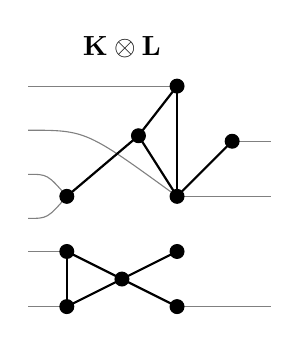
\begin{tikzpicture}[scale=0.7]
    \GraphInit[vstyle=Classic]
    \SetUpEdge[style=-]
    \SetVertexMath
    \tikzset{VertexStyle/.style = {shape=circle, fill=black, minimum size=5pt, inner sep=1pt, draw}}

\def\wirelen{0.7}
    \def\xsh{1}
    \def\ysh{2}

    \node at (1, \ysh+2.7) {$\mathbf{K} \otimes \mathbf{L}$};

\draw[thin, color=gray] (-\wirelen,\ysh-0.4) .. controls (-\wirelen/2,\ysh-0.4) .. (0,\ysh+0);
    \draw[thin, color=gray] (-\wirelen,\ysh+0.4) .. controls (-\wirelen/2,\ysh+0.4) .. (0,\ysh+0);
    \draw[thin, color=gray] (-\wirelen,\ysh+2) -- (2,\ysh+2);
    \draw[thin, color=gray] (2,\ysh+0) -- (3+\wirelen,\ysh+0);
    \draw[thin, color=gray] (3,\ysh+1) -- (3+\wirelen,\ysh+1);
    \draw[thin, color=gray] (-\wirelen,\ysh+1.2) .. controls (\wirelen/2,\ysh+1.2) .. (2,\ysh);

    \Vertex[x=1.3,y=\ysh+1.1,NoLabel]{ax1}
    \Vertex[x=0,y=\ysh+0,NoLabel]{a2}
    \Vertex[x=2,y=\ysh+2,NoLabel]{b2}
    \Vertex[x=2,y=\ysh+0,NoLabel]{c2}
    \Vertex[x=3,y=\ysh+1,NoLabel]{e2}

    \Edges(a2,ax1,b2,c2)
    \Edges(c2,e2)

    \Edge(c2)(ax1)

\draw[thin, color=gray] (\xsh+1+\wirelen+1,0) -- (\xsh+1,0);
    \draw[thin, color=gray] (\xsh+-1,0) -- (\xsh-1-\wirelen,0);
    \draw[thin, color=gray] (\xsh+-1,1) -- (\xsh-1-\wirelen,1);

    \Vertex[x=\xsh+1,y=0,NoLabel]{a3}
    \Vertex[x=\xsh+1,y=1,NoLabel]{b3}
    \Vertex[x=\xsh-1,y=0,NoLabel]{c3}
    \Vertex[x=\xsh-1,y=1,NoLabel]{e3}

    \Vertex[x=\xsh+0,y=0.5,NoLabel]{bx3}

    \Edges(e3,c3,b3)
    \Edge(e3)(a3)
\end{tikzpicture}
     \end{subfigure}
    \hspace{0.6cm}
    \begin{subfigure}{0.25\textwidth}
        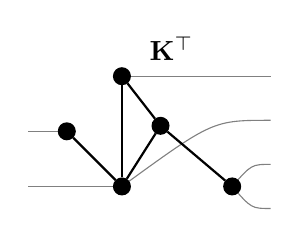
\begin{tikzpicture}[scale=0.7]
    \GraphInit[vstyle=Classic]
    \SetUpEdge[style=-]
    \SetVertexMath

    \def\wirelen{0.7}
\begin{scope}[xscale=-1]
\draw[thin, color=gray] (-\wirelen,-0.4) .. controls (-\wirelen/2,-0.4) .. (0,0);
        \draw[thin, color=gray] (-\wirelen,0.4) .. controls (-\wirelen/2,0.4) .. (0,0);
        \draw[thin, color=gray] (-\wirelen,2) -- (2,2);
        \draw[thin, color=gray] (2,0) -- (3+\wirelen,0);
        \draw[thin, color=gray] (3,1) -- (3+\wirelen,1);
        \draw[thin, color=gray] (-\wirelen,1.2) .. controls (\wirelen/2,1.2) .. (2,0);

        \Vertex[x=1.3,y=1.1,NoLabel]{ax1}
        \Vertex[x=0,y=0,NoLabel]{a2}
        \Vertex[x=2,y=2,NoLabel]{b2}
        \Vertex[x=2,y=0,NoLabel]{c2}
        \Vertex[x=3,y=1,NoLabel]{e2}

        \Edges(a2,ax1,b2,c2)
        \Edges(c2,e2)


        \Edge(c2)(ax1)

    \end{scope}
    \node at (-1.1,2.5) {$\mathbf{K}^\top$};
\end{tikzpicture}
         \vspace{1cm}
    \end{subfigure}
    \end{center}
    \caption{Operations on gadgets $\vk \in \mathfrak{G}(4,2)$ and $\mathbf{L} \in \mathfrak{G}(2,1)$. 
        Dangling edges are drawn thinner than internal edges.}
    \label{fig:gadgetops}
\end{figure}

\begin{definition}[$\langle\cdot,\cdot\rangle,\|\cdot\|$]
    For $n$-ary gadgets $\vk$ and $\vl$, construct the signature grid
    $\langle \vk,\vl \rangle$ by connecting the $i$th dangling edges
    of $\vk$ and $\vl$, for $i \in [n]$.
    If $\vk$ and $\vl$ have signatures $K$ and $L$, then define $\langle K,L \rangle
    := \holant_{\langle \vk,\vl\rangle} = \langle K^{n,0}, L^{n,0}\rangle$ (the standard
    inner product on $\rr^{q^n}$). Define $\|F\| := \sqrt{\langle F,F\rangle} = \sqrt{\sum_{\vx} F_{\vx}^2}$.
\end{definition}

\subsection{Signature Transformations and Invariance}
\begin{definition}[$T(\rr^q)$]
    Following Schrijver \cite{schrijver_tensor_2008}, define
    \[
        T(\rr^q) := \bigcup_{n \in \mathbb{N}} (\rr^q)^{\otimes n}
    \]
    to be the set of all signatures on domain $[q]$.
\end{definition}

\begin{definition}[$HF,H\fc$]
    Define an action of the group $\text{GL}_q(\rr)$ of invertible $q \times q$ matrices on the set 
    $T(\rr^q)$ by, for $H \in \text{GL}_q(\rr)$ and 
    $F \in (\rr^q)^{\otimes n}$, letting $HF\in (\rr^q)^{\otimes n}$ be the signature whose signature vector is
    $H^{\otimes n}f$ -- that is, $(HF)^{n,0} = H^{\otimes n}f$.

    For a signature set $\fc \subset T(\rr^q)$, define $H\fc := \{HF \mid F \in \fc\}$.
\end{definition}
We usually have $H \in O(q)$, the $q \times q$ (real) orthogonal group. We will use the following
notations from invariant theory \cite{schrijver_tensor_2008, regts_rank_2012}.
\begin{definition}[$T(\rr^q)^Q$, $\stab(\fc)$]
    \label{def:invariance}
    For a subgroup $Q \subset O(q)$, define
    \[
        T(\rr^q)^Q := \{F \in T(\rr^q) \mid HF = F \text{ for every } H \in Q\} \subset T(\rr^q).
    \]
    Dually, for a signature set $\fc \subset T(\rr^q)$, define
    \[
        \stab(\fc) := \{H \in O(q) \mid HF = F \text{ for every } F \in \fc\} \subset O(q).
    \]
\end{definition}
A two-sided dangling edge, or \emph{wire}, has no incident vertices. As a gadget with one
left-facing and one right-facing dangling end, a wire
has siganture matrix $I$ (the identity), as its left and right inputs must agree.
Connecting the two ends of a wire, we obtain a vertexless loop.
\begin{definition}[$\mathcal{W}$]
    Let $\mathcal{W} \subset T(\rr^q)$ be the signatures of
    gadgets with no vertices -- that is, the signatures of gadgets consisting of only wires and 
    vertexless loops.
\end{definition}
A gadget consisting of $n$ wires has a $2n$-ary
signature in $\mathcal{W}$, which uniquely corresponds, via the order of the gadget's dangling edges,
to a partition (or matching) of $[2n]$ into two-element subsets.
Since the gadgets defining $\mathcal{W}$ have no vertices, they belong to $\gk$ for any $\fc$.
This view of $\mathcal{W}$ as a set of universal signatures is reinforced by the following
classical theorem from representation theory, called the (tensor) \emph{First Fundamental Theorem} for
$O(q)$, proved by Weyl \cite{weyl_classical_1966}, and stated in this
form by Regts \cite[Theorem 4.3]{regts}. 
Define $\langle \fc \rangle_+$ as the set of all $\rr$-linear 
combinations of (matching-arity) signatures in $\fc$.
\begin{theorem}[FFT for $O(q)$]
    $T(\rr^q)^{O(q)} = \langle \mathcal{W} \rangle_+$.
    \label{thm:fft}
\end{theorem}
We will not need the $\subseteq$ direction of \autoref{thm:fft}, although it follows directly from
our \autoref{thm:intertwiner_gadget} below. The $\supseteq$ direction follows from a simple calculation
and has the geometric intuition shown in \autoref{fig:fft}.
\begin{figure}[ht!]
    \centering
    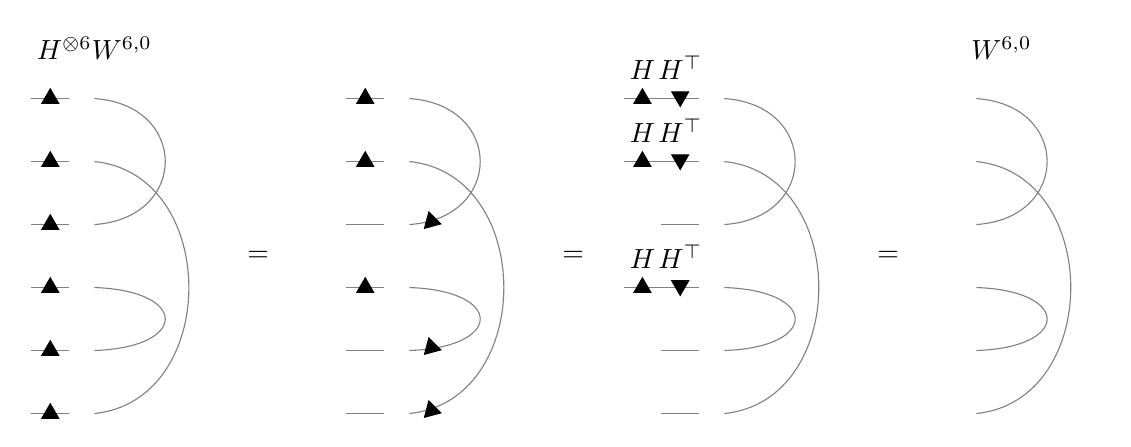
\begin{tikzpicture}[scale=0.8]
    \tikzset{VertexStyle/.style = {shape=circle, fill=black, minimum size=5pt, inner sep=1pt, draw}}
    \GraphInit[vstyle=Classic]
    \SetUpEdge[style=-]
    \SetVertexMath

\def\dx{2}

    \node at (\dx+2.6, 2.5) {$=$};
    \node at (3.5*\dx+2.6, 2.5) {$=$};
    \node at (6*\dx+2.6, 2.5) {$=$};

    \node at (\dx, 5.8) {$H^{\otimes 6} W^{6,0}$};
    \node at (8*\dx+0.4, 5.8) {$W^{6,0}$};

    \foreach \iy in {0,1,...,5} {
        \draw[thin, color=gray] (\dx-1,\iy) -- (\dx-0.4,\iy);
        \node[draw, fill=black, regular polygon, regular polygon sides=3, minimum size = 7pt, inner sep = 1pt] at (\dx-0.7,\iy) {};
    };

    \foreach \ix in {1,3.5,6,8} {
        \draw[thin, color=gray] (\dx*\ix,3) .. controls (\dx*\ix+1.5,3.1) and (\dx*\ix+1.5,4.9) .. (\dx*\ix,5);
        \draw[thin, color=gray] (\dx*\ix,0) .. controls (\dx*\ix+2,0.2) and (\dx*\ix+2,3.8) .. (\dx*\ix,4);
        \draw[thin, color=gray] (\dx*\ix,1) .. controls (\dx*\ix+1.5,1.05) and (\dx*\ix+1.5,1.95) .. (\dx*\ix,2);
    };

    \foreach \iy in {2,4,5} {
        \draw[thin, color=gray] (3.5*\dx-1,\iy) -- (3.5*\dx-0.4,\iy);
        \node[draw, fill=black, regular polygon, regular polygon sides=3, minimum size = 7pt, inner sep = 1pt] at (3.5*\dx-0.7,\iy) {};
    };
    \foreach \iy in {0,1,3} {
        \draw[thin, color=gray] (3.5*\dx-1,\iy) -- (3.5*\dx-0.4,\iy);
        \node[draw, fill=black, rotate=15, regular polygon, regular polygon sides=3, minimum size = 7pt, inner sep = 1pt] at (3.5*\dx+0.35,\iy+0.05) {};
    };

    \foreach \iy in {0,1,3} {
        \draw[thin, color=gray] (6*\dx-1,\iy) -- (6*\dx-0.4,\iy);
    };
    \foreach \iy in {2,4,5} {
        \draw[thin, color=gray] (6*\dx-1.6,\iy) -- (6*\dx-0.4,\iy);
        \node[draw, fill=black, regular polygon, regular polygon sides=3, minimum size = 7pt, inner sep = 1pt, label={[label distance=-0.2mm]$H$}] at (6*\dx-1.3,\iy) {};
        \node[draw, fill=black, rotate=180, regular polygon, regular polygon sides=3, minimum size = 7pt, inner sep = 1pt, label={[label distance=0.2mm]below:$H^\top$}] at (6*\dx-0.7,\iy+0.03) {};
    };
\end{tikzpicture}

     \caption{Demonstrating $H^{\otimes 6}W^{6,0} = W^{6,0}$ for 6-ary $W \in \mathcal{W}$ and
    orthogonal $H$. Each lower $H$ is moved
    along its wire to the top, and transposed in the process (its left and
right dangling edges are switched).}
    \label{fig:fft}
\end{figure}

\subsection{The Holant Theorem}
\label{sec:holanttheorem}
Throughout this work, we will be considering pairs of signature sets, usually denoted $\fc$
and $\gc$. We assume such pairs are \emph{similar}, meaning they have the same domain size $q$ and
there is a bijection $\fc \to \gc$ such that, for $n$-ary $F \in \fc$, the image $G \in \gc$ of $F$, 
called the signature \emph{corresponding} to $F$ and denoted by $F \leftrightsquigarrow G$, has the same
arity $n$.
\begin{definition}[$\vk_{\fc\to\gc}, \Omega_{\fc\to\gc}$]
    For (similar) sets $\fc$ and $\gc$ and gadget $\vk \in \gk$, define the gadget
    $\vk_{\fc\to\gc} \in \mathfrak{G}_{\gc}$ by replacing every $F \in \fc$ assigned to a vertex in
    $\vk$ with the corresponding $G \in \gc$. If $\vk$ has zero dangling edges then it is an
    $\fc$-grid $\Omega$, and is transformed to a $\gc$-grid $\Omega_{\fc\to\gc}$.
\end{definition}

Holant problems were originally motivated by the following theorem, a powerful reduction tool
proved by Valiant \cite{valiant}.
For $F \in (\rr^q)^{\otimes n}$ and $A \in \text{GL}_q(\rr)$, define $FA$ similarly
to $AF$, by $(FA)^{0,n} = F^{0,n}A^{\otimes n}$.
\begin{theorem}[The Holant Theorem]
    For any $(\fc \mid \fc')$-grid $\Omega$ and matrix $A \in \text{GL}_q(\rr)$,
    \[
        \holant_{\Omega}(\fc \mid \fc') = \holant_{\Omega'}
        (A\fc \mid \fc' A^{-1}),
    \]
    where $\Omega' = \Omega_{(\fc\sqcup\fc') \to (A\fc \sqcup \fc' A^{-1})}$.
    \label{thm:holant}
\end{theorem}
Xia \cite{xia} conjectured that the converse of \autoref{thm:holant} holds as long as one of
$\fc$ or $\fc'$ contain a signature with arity greater than one -- that is, if 
$\holant_{\Omega}(\fc \mid \fc') = \holant_{\Omega_{(\fc\sqcup\fc') \to (\gc \sqcup \gc')}}(\gc \mid \gc')$
for every $(\fc \mid \fc')$-grid $\Omega$, then there is an $A \in \text{GL}_q(\cc)$ 
such that $\gc = A\fc$ and $\gc' = \fc' A^{-1}$. However, Cai and Chen
\cite[Section 7.1.1]{cai_chen_2017} observe that this conjecture is false. They consider the problems
\[
    \holant([0,1,0] \mid [a,b,1,0,0]) ~~\text{and}~~ \holant([0,1,0] \mid [0,0,1,0,0])
\]
for any $a,b$ not both 0,
where $[0,1,0]$ and $[a,b,1,0,0]$ are symmetric signatures on the Boolean domain $\{0,1\}$ 
of arity $n=2,4$, respectively, specified by their values on input strings of Hamming
weight $0$ through $n$.
For both problems, $[0,1,0]$ is only nonzero on edge assignment $\sigma$ if $\sigma$ assigns its two
incident edges opposite values. Thus, unless its contribution to the total Holant value is 0, 
$\sigma$ must assign 0 to exactly half the edges in $\Omega$, and 1 to the other half. Then, since
every $[a,b,1,0,0]$ evaluates to zero
whenever it receives more 1 inputs than 0 inputs, no nonzero assignment $\sigma$ assigns any
$[a,b,1,0,0]$ more 0 inputs than 1 inputs. Therefore, in this context,
$[a,b,1,0,0]$ is indistinguishable from $[0,0,1,0,0]$, so the hypothesis of Xia's conjecture is satisfied. 
However, there is no $A \in \text{GL}_2(\cc)$ satisfying $A[0,1,0] = [0,1,0]$ and 
$[a,b,1,0,0]A^{-1} = [0,0,1,0,0]$. To see this, if $A = \begin{bmatrix} a & b \\ c & d\end{bmatrix}$, then, with the signature vector of $[0,1,0]$ being $(0,1,1,0)^\top$,
\[
    A^{\otimes 2}
    \begin{bmatrix} 0 \\ 1 \\ 1 \\ 0 \end{bmatrix} =
    \begin{bmatrix} 
        a^2 & ab & ba & b^2 \\
        ac & ad & bc & bd \\
        ca & cb & da & db \\
        c^2 & cd & dc & d^2
    \end{bmatrix}
    \begin{bmatrix} 0 \\ 1 \\ 1 \\ 0 \end{bmatrix}
    = \begin{bmatrix} 0 \\ 1 \\ 1 \\ 0 \end{bmatrix}
    \iff ab = cd = 0 \text{ and } ad + bc = 1
    \implies \begin{cases} a = d = 0 & \text{or} \\ b = c = 0\end{cases}.
\]
If $b=c=0$ then $A$ simply rescales a signature's entries, and if $a=d=0$ then
$A$ rescales a signature's entries and exchanges the roles of $0$ and $1$, which has the effect of
reversing the entries in the $[\cdot,\ldots,\cdot]$ notation. Thus $[0,0,1,0,0]A = [0,0,*,0,0]
\neq [a,b,1,0,0]$.

This counterexample exists due to 
the bipartiteness enforced by the definition of $\holant(\fc \mid \gc)$, because
\[
    \left\langle [0,0,1,0,0],[0,0,1,0,0]\right\rangle = \|[0,0,1,0,0]\|^2
    \neq \|[a,b,1,0,0]\|^2 = \left\langle [a,b,1,0,0],[a,b,1,0,0] \right\rangle,
\]
so $[a,b,1,0,0]$ and $[0,0,1,0,0]$ are not indistinguishable on
general (non-bipartite) signature grids. To avoid such counterexamples, we consider the
following well-known form of \autoref{thm:holant} that applies to non-bipartite grids.
An edge in an $\fc$-grid $\Omega$, viewed on its own, is a wire,
with signature $I$. Therefore we can, without changing the Holant value, replace each edge in 
$\Omega$ by a binary gadget with a single vertex assigned $I$, effectively splitting the edge into a path
of length two. Then $\Omega$ is a signature grid in the context of
$\holant(\fc \mid I)$, so, by \autoref{thm:holant}, for any invertible $H$,
$\holant_\Omega(\fc \mid I) = \holant_{\Omega'}(H\fc \mid IH^{-1})$. If $H$ is orthogonal,
then, by \autoref{thm:fft}, $I^{0,2}H^{-1} = (HI^{2,0})^\top = (I^{2,0})^\top = I^{0,2}$, so
$\holant_\Omega(\fc \mid I) = \holant_{\Omega'}(H\fc \mid I)$. Then $\holant(H\fc \mid I)$
is again equivalent to $\holant(H\fc)$, so we have proved the following.
\begin{corollary}[The Orthogonal Holant Theorem]
    \label{cor:holanttheorem}
    If $\gc = H\fc$ for orthogonal matrix $H$, then $\holant_\Omega(\fc) = \holant_{\Omega_{\fc\to\gc}}(\gc)$ for every $\fc$-grid $\Omega$.
\end{corollary}
Xia \cite{xia} also considers the converse of \autoref{cor:holanttheorem}, and proves that it holds
for specific $\fc$ and $\gc$ consisting of real-valued symmetric signatures with small domain
and/or arity.
The main result of this work is the converse of \autoref{cor:holanttheorem} for any
sets $\fc$ and $\gc$ of real-valued signatures, with no restrictions.
\begin{theorem}[Main Result]
    \label{thm:result}
    Let $\fc$, $\gc$ be sets of real-valued signatures. Then the following are equivalent.
    \begin{enumerate}[label=(\roman*)]
        \item $\holant_{\Omega}(\fc) = \holant_{\Omega_{\fc\to\gc}}(\gc)$
        for every $\fc$-grid $\Omega$.
        \item There is a real orthogonal matrix $H$ such that $H\fc = \gc$.
    \end{enumerate}
\end{theorem}
Call $\fc$ and $\gc$ satisfying (i) \emph{Holant-indistinguishable}, and call $\fc$ and
$\gc$ satisfying (ii) \emph{ortho-equivalent}. 
The following two properties follow directly from the definitions and \autoref{cor:holanttheorem},
but, as they will
prove useful throughout the proof of \autoref{thm:result}, we state them explicitly.
\begin{proposition}
    For any orthogonal $H_1$ and $H_2$, $\fc$ and $\gc$ are 
    ortho-equivalent/Holant-indistinguishable if and only if
    $H_1\fc$ and $H_2\gc$ are ortho-equivalent/Holant-indistinguishable, respectively.
    \label{prop:transform}
\end{proposition}
\begin{proposition}
    For any $\fc$ and $\gc$, and any additional pair $\fc'$ and $\gc'$ of signature sets,
    if $\fc \sqcup \fc'$ and $\gc \sqcup \gc'$ are ortho-equivalent (where the $\fc'$ signatures in $\fc \sqcup \fc'$ correspond to the $\gc'$ signatures in $\gc \sqcup \gc'$), then $\fc$ and $\gc$ are ortho-equivalent.
    \label{prop:union}
\end{proposition}   

\subsection{Block Matrices and Signatures}
\label{sec:block}
\begin{definition}
    \label{def:block}
    Let $\ic$ be an index/domain set, and $X \sqcup Y = \ic$ be a nontrivial partition of $\ic$.
    \begin{enumerate}
    \item
    For a matrix $H \in \rr^{\ic \times \ic}$ and $R,C \in \{X,Y\}$, let $H|_{R,C} \in \rr^{R\times C}$ be the
    submatrix of $H$ with rows indexed by $R$ and columns indexed by $C$. Up to row and
    column reordering, $H$ is the block matrix
    \[
        H = \begin{bmatrix} H|_{X,X} & H|_{X,Y} \\ H|_{Y,X} & H|_{Y,Y}\end{bmatrix}.
    \]
    \item
    More generally, for a signature/tensor $F \in \rr^{\ic^n}$ and $\vr \in \{X,Y\}^n$, define
    $F|_{\vr} \in \rr^{\vr}$ (where we identify $\vr$ with the set $\prod_{i=1}^n R_i$) to be the subtensor of $F$ with $i$th
    input restricted to $R_i$.
    For signature set $\fc$, let $\fc|_{\vr} := \{F|_{\vr}: F \in \fc\}$.

    Abbreviate $F|_X := F|_{X^n}$ and $\fc|_X := \fc|_{X^n}$.
    \item 
    Let $F^{m,d} \in \rr^{\ic^m \times \ic^d}$ be a signature matrix, and let 
    $\vr \in \{X,Y\}^m$ and $\vc \in \{X,Y\}^d$. Define 
    $F^{m,d}|_{\vr,\vc} \in \rr^{\vr \times \vc}$
    as the submatrix of $F^{m,d}$ with rows indexed by $\vr$ and columns indexed by
    $\vc$ (in other words, $F^{m,d}|_{\vr,\vc} = (F|_{\vr\vc})^{m,d}$, where
    $\vr\vc$ is the concatenation of $\vr$ and $\vc$).
    \end{enumerate}
\end{definition}

\begin{definition}[$\oplus$]
\label{def:oplus-f-g}
    Let $F,G$ be $n$-ary signatures on domains $V(F)$, $V(G)$, both of size $q$.
    The \emph{direct sum} $F \oplus G$ of $F$ and $G$ is an
    $n$-ary signature on domain $V(F) \sqcup V(G)$ defined by
    \[
        (F \oplus G)_{\vx} = \begin{cases} 
            F_{\vx} & \vx \in V(F)^n \\
            G_{\vx} & \vx \in V(G)^n \\
            0 & \text{otherwise}
        \end{cases}
        \qquad\text{for } \mathbf{x} \in (V(F) \sqcup V(G))^n.
    \]
    For signature sets $\fc$ and $\gc$, define 
    $\fc \oplus \gc = \{F \oplus G \mid \fc \ni F \leftrightsquigarrow G \in \gc\}$.
\end{definition}
We will frequently apply \autoref{def:block} to the partition $V(\fc) \sqcup V(\gc)$ of the domain
of $\fc\oplus\gc$.
It follows directly from the definitions that, for $\fc \ni F \leftrightsquigarrow G \in \gc$ and any 
$m+d = \arity(F)$,
\begin{equation}
    (F \oplus G)^{m,d}|_{\vr,\vc} = 
    \begin{cases}
        F^{m,d} & \vr = V(\fc)^m \wedge \vc = V(\fc)^d \\ G^{m,d} & \vr = V(\gc)^m \wedge \vc = V(\gc)^d \\ 0 & \text{otherwise}.
    \end{cases}
    \label{eq:oplus_index}
\end{equation}
\autoref{sec:appendix_block} states and proves some additional necessary results involving 
actions of block matrices on block signatures.
These additional results confirm that these block structures interact as
one would expect, analogously to ordinary block matrix algebra.
 \section{Quantum Gadget Duality}
\label{sec:duality}
In this section, we prove a duality (\autoref{thm:intertwiner_gadget}) between tensors invariant
under the action of $\stab(\fc)$ and the signatures of $\fc$-gadgets. 
\autoref{thm:intertwiner_gadget} and its proof are extensions of Regts' 
\cite[Theorem 3]{regts_rank_2012}
from edge-coloring models to general signature sets $\fc$, largely translated into the language of
signature matrices (see \autoref{lem:tcwd}). This translation
reveals that \autoref{thm:intertwiner_gadget} and its proof are also nonplanar/nonquantum, orthogonal 
versions of similar results of Man\v{c}inska, Roberson, Cai and Young 
\cite{planar,cai_planar_2023,young2022equality} -- see \autoref{rem:duality}.

Say $\fc \subset T(\rr^q)$ is a \emph{graded subalgebra} of $T(\rr^q)$ if 
$\fc \cap (\rr^q)^{\otimes n}$ (the signatures of arity $n$) 
is a vector space over $\rr$ (closed under $\rr$-linear combinations) and
$\fc$ is closed under $\otimes$.
Say $\fc$ is \emph{contraction-closed} if, for every $n$-ary $F \in \fc$,
the $(n-2)$-ary signature resulting from \emph{contracting} any two inputs of $F$ 
(connecting the corresponding dangling edges of the $n$-ary gadget consisting of a single vertex
assigned $F$) is also in $\fc$.
The following theorem, due to Schrijver, is the key connection between
algebra and combinatorics underlying
our proof of \autoref{thm:intertwiner_gadget} and, eventually, \autoref{thm:result}.
\begin{theorem}[{\cite[{Corollary 1e}]{schrijver_tensor_2008}}]
    Let $\fc \subset T(\rr^q)$. Then there is a subgroup $Q \subset O(q)$ with $\fc = T(\rr^q)^Q$
    if and only if $\fc$ is a contraction-closed graded subalgebra of $T(\rr^q)$ containing $I$.
    \label{thm:duality}
\end{theorem}
Schrijver's statement of \autoref{thm:duality} requires that
$\fc$ be ``nondegenerate'', but it can be seen from the proof that
it suffices to assume that $\fc$ contains $I$ (cf. Regts' restatement
\cite[Theorem 4]{regts_rank_2012}).

\begin{definition}[$M(\fc),M(T(\rr^q))$]
    Let $\fc \subset T(\rr^q)$ be a signature set. Define 
    \[
        M(\fc) := \bigcup_{F \in \fc}\left(\bigcup_{\substack{m,d \in \mathbb{N} \\ m+d=\arity(F)}} 
        F^{m,d}\right)
    \]
    to be the set of all flattenings of all tensors in $\fc$. In particular,
    \[
        M(T(\rr^q)) = \bigcup_{m,d \in \mathbb{N}} \rr^{q^m\times q^d}.
    \]
\end{definition}
For a subset $P \subset M(T(\rr^q))$, define $\tcwd{P} \subset M(T(\rr^q))$ to be the set generated
by $P$ under $\circ, \otimes, \top$, and $\rr$-linear combinations of matrices with matching
dimensions.

\begin{definition}[$S_\sigma, S$]
    For permutation $\sigma \in S_n$, define the $2n$-ary \emph{braid} signature $S_\sigma \in \mathcal{W}$ 
    by $(S_\sigma)_{\vx\vy} = 1$ iff $x_i = y_{\sigma(i)}$ for every $i \in [n]$, and 
    $(S_\sigma)_{\vx\vy} = 0$ otherwise.

    Define the 4-ary `swap' signature $S := S_{(01)}$. See \autoref{fig:braid}
\end{definition}
\begin{figure}[ht!]
    \centering
    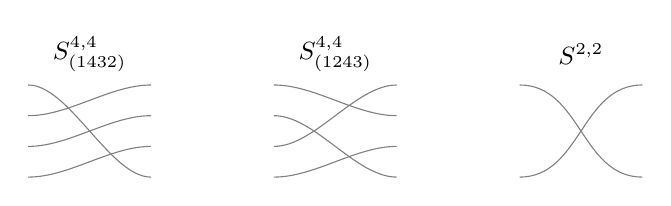
\begin{tikzpicture}[scale=.78]
    \tikzstyle{every node}=[font=\small]
    \GraphInit[vstyle=Classic]
    \SetUpEdge[style=-]
    \SetVertexMath

\def\ysh{0.5}
    \def\xsh{4}
    \def\slen{2}

\node at (\slen/2, 5*\ysh) {$S^{4,4}_{(1 4 3 2)}$};
    \foreach \ll/\rr in {4/1,3/4,2/3,1/2} {
        \draw[thin, color=gray] (0,\ll*\ysh) .. controls
        +(\slen/3,0) and +(-\slen/3,0)..
        (\slen,\rr*\ysh);
    };

    \node at (\xsh+\slen/2, 5*\ysh) {$S^{4,4}_{(1 2 4 3)}$};
    \foreach \ll/\rr in {4/3,3/1,2/4,1/2} {
        \draw[thin, color=gray] (\xsh,\ll*\ysh) .. controls
        +(\slen/3,0) and +(-\slen/3,0)..
        (\xsh+\slen,\rr*\ysh);
    };

    \node at (2*\xsh+\slen/2, 5*\ysh) {$S^{2,2}$};
    \foreach \ll/\rr in {1/4,4/1} {
        \draw[thin, color=gray] (2*\xsh,\ll*\ysh) .. controls
        +(\slen/2,0) and +(-\slen/2,0)..
        (2*\xsh+\slen,\rr*\ysh);
    };

\end{tikzpicture}
     \caption{Braid gadgets and their signature matrices.}
    \label{fig:braid}
\end{figure}
Every permutation is a product of adjacent transpositions, so
$S_\sigma^{n,n} \in \tcwdn{I,S^{2,2}}$ \cite[Lemma 3]{young2022equality}.
The following is a central object of study in the works of
Man\v{c}inska, Roberson, Cai and Young \cite{planar, cai_planar_2023, young2022equality}. 
\begin{definition}
\label{def:tcwd}
For $C \subset M(T(\rr^q))$, define $C(m,d) := C \cap \rr^{q^m\times q^d}$.
$C$ is a \emph{tensor category with duals} (TCWD) if it satisfies the following properties:
\begin{enumerate}[label=(\roman*)]
    \item For fixed $m$ and $d$, $C(m,d)$ is a vector space over $\rr$,
    \item $C$ is closed under $\circ, \otimes, \top$,
    \item $I \in C(1,1)$,
    \item $I^{0,2} \in C(0,2)$.
\end{enumerate}
$C$ is a \emph{symmetric} tensor category with duals if it also satisfies
\begin{enumerate}[label=(\roman*),start=5]
    \item $S^{2,2} \in C(2,2)$.
\end{enumerate}
\end{definition}

We next translate \autoref{thm:duality} into the language of TCWDs by flattening
$\fc$. 
\begin{lemma}
    \label{lem:tcwd}
    A subset $\fc \subset T(\rr^q)$ is a contraction-closed graded subalgebra of $T(\rr^q)$ containing
    $I$ if and only if $M(\fc)$ is a symmetric tensor category with duals.
\end{lemma}
\begin{proof}\textcolor{red}{TOPROVE 0}\end{proof}

Define an action of $O(q)$ on $M(T(\rr^q))$ by 
\[
    HF^{m,d} := H^{\otimes m} F^{m,d} (H^\top)^{\otimes d}.
\]
Using this action, define the matrix version of \autoref{def:invariance}: for $Q \subset O(q)$ and
$\fc \subset T(\rr^q)$,
\begin{align*}
    &M(T(\rr^q))^Q := \{F^{m,d} \in M(T(\rr^q)) \mid H^{\otimes m} F^{m,d} (H^\top)^{\otimes d} = F^{m,d} \text{ for every } H \in Q\} \text{ and}\\
    &\stab(M(\fc)) := \{H \in O(q) \mid H^{\otimes m}F^{m,d} (H^\top)^{\otimes d} = F^{m,d} \text{ for every } F^{m,d} \in M(\fc)\}. 
\end{align*}
The next proposition shows that the matrix and signature versions of these definitions agree.
\begin{proposition}
    \label{prop:invariant_tcwd}
    ~
    \begin{enumerate}
        \item For any subgroup $Q \subset O(q)$, $M(T(\rr^q))^Q$ is a symmetric tensor category with duals.
        \item For any signature $F$ and orthogonal $H$,
            $(HF)^{m,d} = H^{\otimes m} F^{m,d} (H^\top)^{\otimes d}$ for any $m,d$.
        \item $\stab(\fc) = \stab(M(\fc))$. 
    \end{enumerate}
\end{proposition}
\begin{proof}\textcolor{red}{TOPROVE 1}\end{proof}
That part 2 of \autoref{prop:invariant_tcwd} holds for any, not necessarily orthogonal, matrix $A$
is a well-known fact, with a geometric intuition similar to \autoref{fig:fft}. We gave the above
proof to mirror the proof of Cai and Young's similar \cite[Lemma 6]{cai_planar_2023} for quantum
orthogonal matrices, and to highlight the role of $I^{0,2}$ 
in the invariance of a TCWD under edge pivoting (or taking \emph{duals} --
see e.g. \cite[Appendix D]{cai_planar_2023}).

\begin{definition}[$\qk(m,d), \overline{\fc}$]
    \label{def:quantum_gadget}
    A \emph{$(m,d)$-quantum $\fc$-gadget} is a formal (finite) $\rr$-linear combination of gadgets in
    $\gk(m,d)$. Let $\qk(m,d)$ be the collection of all $(m,d)$-quantum $\fc$-gadgets,
    and $\qk = \bigcup_{m,d}\qk(m,d)$.

    Extend the signature matrix function $M$ linearly to $\qk$. Then define the \emph{quantum gadget
    closure} $\ofc$ of $\fc$ as the
    set of signatures obtainable from $\fc$ by quantum gadget construction:
    \[
        \ofc = \bigsqcup_{F^{m,d} \in M(\qk)}F.
    \]
\end{definition}
We use the disjoint union $\sqcup$ because different quantum gadgets could yield the same
signature, and so that, if sets $\fc$ and $\gc$ are similar, then $\ofc$ and
$\ogc$ are similar, with the signature of $\vk \in \qk$ corresponding to the signature of
$\vk_{\fc\to\gc} \in \mathfrak{Q}_{\gc}$.

Since $I,S \in \mathcal{W} \subset \ofc$ for any $\fc$, and $\gk$ is closed under gadget 
$\circ,\otimes$, and $\top$, $M(\qk) = M(\ofc)$ is a symmetric TCWD. Specifically,
the next proposition, which is very similar to \cite[Theorem 3]{young2022equality} (the main difference 
being that we do not assume $\eq \subset \fc$), shows that $M(\qk)$ is the symmetric TCWD generated by $M(\fc)$.
\begin{proposition}
    $M(\qk) = \tcwd{\big\{I,I^{0,2},S^{2,2}\big\} \cup \big\{f \mid F \in \fc\big\}}$.
    \label{prop:mqf}
\end{proposition}
\begin{proof}\textcolor{red}{TOPROVE 2}\end{proof}

\begin{proposition}
    \label{prop:stabfc}
    $\stab(\fc) = \stab(M(\qk)) = \stab(\overline{\fc})$.
\end{proposition}
\begin{proof}\textcolor{red}{TOPROVE 3}\end{proof}

Now we come to the main result of this section. We follow Regts' proof
for the special case of edge coloring models \cite[Theorem 6.8]{regts}.
\begin{theorem}
    \label{thm:intertwiner_gadget}
    Let $\fc$ be a set of real-valued signatures on domain $[q]$. Then
    \[
        T(\rr^q)^{\stab(\fc)} = \ofc.
    \]
    Equivalently, by flattening both sides and applying part 3 of \autoref{prop:invariant_tcwd},
    we have, for any $m,d$,
    \[
        \left(\rr^{q^m\times q^d}\right)^{\stab(\fc)} = M(\qk(m,d)).
    \]
\end{theorem}
\begin{proof}\textcolor{red}{TOPROVE 4}\end{proof}
A direct consequence is the FFT for $O(q)$. Schrijver \cite{schrijver_tensor_2008} gives another 
proof based on \autoref{thm:duality}.
\begin{proof}\textcolor{red}{TOPROVE 5}\end{proof}

\begin{remark}
    \label{rem:duality}
    The reasons we translated from 
    Schrijver and Regts \cite{schrijver_tensor_2008, regts_rank_2012}'s language of
    contraction-closed graded subalgebras to
    Man\v{c}inska, Roberson, Cai and Young
    \cite{planar, cai_planar_2023, young2022equality}'s language of symmetric TCWDs are twofold. 
    The first is to highlight the similarities
    between this section's results and the results of the latter group. 
Replacing $O(q)$ with $S_q$ (the symmetric group of permutation matrices) or $S^+_q$ 
    (the \emph{quantum symmetric group}), enforcing that
    the TCWDs contain $M(\eq)$ (corresponding to quantum gadgets in the context of $\csp$), 
    and dropping the symmetry condition on the TCWDs 
    in the second case (corresponding to quantum gadget planarity), we find our constructions 
    and theorems in this section analogous to those of
    \cite{young2022equality} or \cite{planar, cai_planar_2023}, respectively. In particular, 
    $\stab(\fc)$ becomes $\aut(\fc)$ (the automorphism group of $\fc$ 
    \cite{young2022equality}) or $\qut(\fc)$ (the \emph{quantum automorphism group} of $\fc$
    \cite{planar, cai_planar_2023}), respectively. Then
    $M(T(\rr^q))^{\stab(\fc)}$ becomes the
    \emph{intertwiner space} of $\qut(\fc)$ or $\aut(\fc)$. Applying \autoref{lem:tcwd},
    we find \autoref{thm:duality} perfectly analogous to the
    \emph{Tannaka-Krein duality} used by \cite{young2022equality} and \cite{planar, cai_planar_2023}
    to prove results analogous to \autoref{thm:intertwiner_gadget}.
    As in this work, \cite{planar,cai_planar_2023,young2022equality} use their versions of
    \autoref{thm:intertwiner_gadget} to prove their respective versions of \autoref{thm:result}, but
    due to the nature of $O(q)$ -- in particular, $O(q)$ has no construction analogous to the
    \emph{orbits} and \emph{orbitals} of $S_q$ and $S_q^+$ -- we take a different route for the rest
    of the proof of \autoref{thm:result}.

    The second reason is that, just as the main result of \cite{cai_planar_2023} is a planar, quantum
    version
    of the main result of \cite{young2022equality}, our \autoref{thm:result} should have a planar, 
    quantum
    version (see \autoref{con:quantum} below). Arbitrary contractions do not respect planarity, but,
    by simply removing the symmetry condition (i.e. removing $S^{2,2}$ in \autoref{prop:mqf}), 
    we easily enforce planarity in the language of TCWDs.
\end{remark}

The following lemma is this section's main contribution to proving \autoref{thm:result}, and is the
only nonconstructive step in the proof.
\begin{lemma}
    If $\fc$ and $\gc$ are Holant-indistinguishable, then there is an
    $H \in \stab(\fc \oplus \gc)$ with $H|_{V(\fc),V(\gc)} \neq 0$ or $H|_{V(\gc),V(\fc)} \neq 0$.
    \label{lem:offdiagblock}
\end{lemma}
\begin{proof}\textcolor{red}{TOPROVE 6}\end{proof}
 \section{Domain Induction: The Proof of \autoref{thm:result}}
The following definition and its applications below borrow a simple but powerful idea of Shao and
Cai \cite[Section 8.2]{shao}: isolating all vertices of an
$\fc \cup \{F\}$-grid $\Omega$ assigned $F$, the rest of $\Omega$ is an $\fc$-gadget. 
If adding certain $F$ to $\fc$ and $G$ to $\gc$ simplifies the proof of ortho-equivalence,
we use the subgadget perspective to obtain Holant-indistinguishability of $\fc\cup\{F\}$
and $\gc\cup\{G\}$ from the Holant-indistinguishability of $\fc$ and $\gc$.
\begin{definition}[Subgadget, $\overline{\vk}$]
    Let $\vj$ be a gadget. A \emph{subgadget} $\vk \subset \vj$ induced by a subset $U \subset V(\vj)$ 
    of vertices of $\vj$ is a gadget composed of the vertices in $U$ and 
    \emph{all} of their incident edges: internal edges of $\vj$ incident to 
    exactly one vertex in $U$ become new dangling edges of $\vk$.
    For any $\vk \subset \vj$, there is a
    unique (up to left/right dangling edge pivoting) $\overline{\vk} \subset\vj$, induced by $V(J) \setminus U$, called the 
    \emph{complement} of $\vk$, such that, upon reconnecting the new dangling edges of $\vk$ and
    $\overline{\vk}$, we recover $\vj$.

    We often take $\vj$ to be a signature grid (0-ary gadget) $\Omega$, in which case
    $\Omega = \left\langle \vk,\overline{\vk} \right\rangle$.
\end{definition}

Say $\fc$ is \emph{quantum-gadget-closed} if $\fc = \ofc$. The following proposition, a
nonplanar, orthogonal version of \cite[Lemmas 31 and 32]{cai_planar_2023}, lets us assume
$\fc$ and $\gc$ are quantum-gadget-closed when proving \autoref{thm:result}.
\begin{lemma}
    \label{prop:closure}
    For any signature sets $\fc$ and $\gc$,
    \begin{enumerate}
        \item $\fc$ and $\gc$ are Holant-indistinguishable iff $\overline{\fc}$ and $\overline{\gc}$ are
            Holant-indistinguishable.
        \item For any orthogonal $H$, $H\fc = \gc$ iff $H\overline{\fc} = \overline{\gc}$.
    \end{enumerate}
\end{lemma}
\begin{proof}\textcolor{red}{TOPROVE 7}\end{proof}

In the context of \#CSP, $\eq$ enables the gadget-construction of entrywise 
products of arbitrary signatures. This is a basis for Vandermonde interpolation, a powerful 
technique in the study of counting problems.
In the general Holant setting, we cannot construct the entrywise product of arbitrary signatures,
but, for binary signatures whose matrix forms are diagonal, composition is equivalent to entrywise
product. We use the following form of Vandermonde interpolation, which follows directly from the similar
\cite[Lemma 2.3]{grohe_homomorphism_2022}.
\begin{proposition}
    \label{prop:vandermonde}
    Let $V \subset \rr^q$ be a vector space closed under entrywise product and containing the
    all-ones vector. For $v \in V$ and $a \in \rr$, define the indicator vector $v^a \in \{0,1\}^q$ by
    $(v^a)_x = 1$ if $v_x = a$ and $(v^a)_x = 0$ otherwise. Then $v^a \in V$ for every
    $v \in V$ and $a \in \rr$.
\end{proposition}
\autoref{prop:vandermonde} will give us the following matrices, whose diagonals we identify
with $\rr^q$:
For $Z \subset [q]$, define the diagonal matrix (binary signature)
$\mathds{1}_Z \in \{0,1\}^{q \times q}$ by $(\mathds{1}_Z)_{x,x} = 1$ if $x \in Z$, and $(\mathds{1}_Z)_{x,x} = 0$ otherwise.
\begin{lemma}
    \label{lem:restriction}
    Let $\fc$ and $\gc$, on domain $[q]$, be Holant-indistinguishable, and let $Z \subset [q]$. If $\fc$ and
    $\gc$ contain corresponding copies of $\mathds{1}_Z$, then $\fc|_Z$ and $\gc|_Z$ are 
    Holant-indistinguishable.
\end{lemma}
\begin{proof}\textcolor{red}{TOPROVE 8}\end{proof}

\begin{lemma}
    \label{lem:induction}
    Let $\fc$ and $\gc$ be signature sets on domain $[q]$, and suppose \autoref{thm:result} holds for
    all $\fc'$, $\gc'$ on domain smaller than $q$. If $\fc$ and $\gc$ are Holant-indistinguishable
    and contain corresponding copies of a diagonal matrix (binary signature)
    $D \not\in \spn(I)$, then $\fc$ and $\gc$ are ortho-equivalent. 
\end{lemma}
\begin{proof}\textcolor{red}{TOPROVE 9}\end{proof}

For any set $S$ of matrices and matrices $A,B$, let $A \circ S \circ B := \{A  Q  B \mid Q \in S\}$.
\begin{proposition}
    For any $\fc$ and orthogonal matrix $H$, 
    $\stab(H\fc) = H \circ \stab(\fc) \circ H^\top$.
    \label{prop:stabbasis}
\end{proposition}
\begin{proof}\textcolor{red}{TOPROVE 10}\end{proof}
The final step is to realize the diagonal matrix $D$ in the statement of \autoref{lem:induction}, and
apply induction.
\begin{proof}\textcolor{red}{TOPROVE 11}\end{proof} 
 \section{Consequences of \autoref{thm:result}}
\label{sec:corollaries}
In this section, we exploit the expressiveness of the Holant framework to show that \autoref{thm:result}
encompasses a variety of existing results, and derive a few novel consequences.
\subsection{Counting CSP and graph homomorphisms}
For signature set $\fc$, define the \emph{counting constraint satisfaction problem} $\csp(\fc)$
with \emph{constraint function} set $\fc$
to be the problem $\holant(\fc \mid \eq)$. Vertices assigned signatures in $\fc$ and $\eq$ are 
\emph{constraints} and \emph{variables}, respectively, and a $(\fc\mid\eq)$-grid $\Omega$ is a 
constraint-variable incidence graph, where a variable appears in all of its incident constraints. Then
$\holant_\Omega(\fc\mid\eq)$ is the sum over all variable assignments of the product of the constraint
evaluations.
Like Holant, $\csp$ is a well-studied
problem in counting complexity, with dichotomy theorems classifying $\csp(\fc)$ as either tractable
or \#P-hard proved for increasingly broad classes of constraint function sets 
\cite{bulatov_2013, dyer_richerby, cai-chen-lu, cai-chen-complexity}. 

By inserting a dummy degree-2 constraint vertex assigned $I = (=_2) \in \eq$ between adjacent variable vertices and combining adjacent constraint
vertices assigned $=_a$ and $=_b$ into a single constraint vertex assigned $=_{a+b-2}$, we see that
$\holant(\fc \cup \eq)$ is equivalent to $\holant(\fc \mid \eq)$. Using a standard Vandermonde
interpolation argument, Xia \cite{xia} shows that $H$ satisfies $H \eq = \eq$ if and only
$H$ is a permutation matrix. If $H\fc = \gc$ for some permutation matrix $H$, then $\fc$ and $\gc$
are the same up to relabeling of their domains, so are isomorphic. 
Now, applying \autoref{thm:result} to $\fc \cup \eq$ and $\gc \cup
\eq$, we obtain the main result of Young \cite{young2022equality} for real-valued constraint functions.
Say that $\fc$ and $\gc$ are $\csp$-indistinguishable if $\fc\cup\eq$ and $\gc\cup\eq$ are 
Holant-indistinguishable (in other words, every $\csp$ instance has the same value whether we use 
constraint functions from $\fc$ or from $\gc$).
\begin{corollary}
    Let $\fc$ and $\gc$ be sets of real-valued constraint functions.
    Then $\fc$ and $\gc$ are isomorphic if and only if $\fc$ and $\gc$ are $\csp$-indistinguishable.
    \label{cor:isomorphism}
\end{corollary}
As discussed in \autoref{sec:holant}, 
$\holant(A_X \mid \eq) = \csp(A_X)$ counts the number of homomorphisms to graph $X$. Therefore
\autoref{cor:isomorphism} is a generalization of the classical theorem of Lovász \cite{lovasz_operations}
that two graphs are isomorphic if and only if they admit the same number of homomorphisms from every
graph.

Let $\eq_2 \subset \eq$ be the set of equality signatures of even arity. 
Schrijver \cite{schrijver_tensor_2008} 
shows\footnote{The First Fundamental Theorem for $S_q^{\pm} \subset O(q)$ (the group of signed
    permutation matrices) states that $T(\rr^q)^{S_q^{\pm}} = \overline{\eq_2}$
    (cf. \autoref{thm:fft}, and recall that $\langle \mathcal{W} \rangle_+ = \overline{\varnothing}$).
    It follows as in the proof of \autoref{thm:intertwiner_gadget} that $\stab(\eq_2) = S_q^{\pm}$.
    The fact that $\stab(\eq) = S_q \subset O(q)$ (the group of permutation matrices) similarly follows
    from the First Fundamental Theorem for $S_q$, which states that
    $T(\rr^q)^{S_q} = \overline{\eq}$.
}
that $H$
satisfies $H\eq_2 = \eq_2$ if and only if $H$ is a signed permutation matrix (a matrix with entries
in $\{0,\pm 1\}$ and exactly one nonzero entry in each row and column). As above,
$\holant(\fc \cup \eq_2)$ is equivalent to $\holant(\fc \mid \eq_2)$ (critically, if $=_a \in \eq_2$
and $=_b \in \eq_2$, then $=_{a+b-2} \in \eq_2$). Then, defining $\csp^2(\fc) := \holant(\fc \mid \eq_2)$ as $\csp(\fc)$
restricted to instances in which every variable appears an even number of times \cite{cai2015holant,huang_2016_dichotomy}, we have
\begin{corollary}
    Let $\fc$ and $\gc$ be sets of real-valued constraint functions.
    Then there is a signed permutation matrix $P$ satisfying $\gc = P\fc$ if and only if
    $\fc$ and $\gc$ are $\csp^2$-indistinguishable.
\end{corollary}
In particular, since (unweighted) graph adjacency matrices $A_X$ and $A_Y$ have entries in $\{0,1\}$,
we have $P^{\otimes 2}(A_X)^{2,0} = (A_Y)^{2,0} \implies 
    (P')^{\otimes 2}(A_X)^{2,0} = (A_Y)^{2,0}$,
where $P'$ is the permutation matrix created by flipping every $-1$ entry of $P$ to $1$. Therefore
we have the following sharpening of Lovász's theorem.
\begin{corollary}
    Graphs $X$ and $Y$ are isomorphic if and only if they admit the same number of homomorphisms
    from those graphs in which all vertices have even degree.
\end{corollary}

\subsection{Simultaneous matrix similarity}
Let $\fc$ and $\gc$ be sets of binary signatures, thought of as matrices. Any connected $\fc$-grid
$\Omega$
is a cycle. Breaking an edge of the cycle, we obtain a binary path gadget with signature matrix
$\prod_{i=1}^c F_i$, where, depending on its orientation, each $F_i \in \fc$ or $F_i^\top \in \fc$.
Connecting the path's two dangling edges, we reform $\Omega$, which thus has Holant value
$\tr\left(\prod_{i=1}^c F_i\right)$. Let $\Gamma_{\fc}$ be the set of all finite products of
matrices in $\fc$ and $\fc^\top := \{F^\top \mid F \in \fc\}$. Define $\Gamma_{\gc}$ similarly and,
for a word $w \in \Gamma_{\fc}$, construct $w_{\fc\to\gc} \in \Gamma_{\gc}$ by replacing every character
$F$ or $F^\top$ in $w$ by the corresponding $G$ or $G^\top$, respectively. 
For orthogonal $H$, we have $H\fc = \gc \iff HF^{1,1} = G^{1,1}H$ for every $F \leftrightsquigarrow G$
(by part 2 of \autoref{prop:invariant_tcwd}), so, in this
setting, \autoref{thm:result} is equivalent to the following real-valued case of a
classical theorem from representation theory, due to Specht \cite{specht} and Wiegmann \cite{wiegmann}.
Grohe, Rattan, and Seppelt \cite{grohe_homomorphism_2022} also give a combinatorial proof.
\begin{corollary}
    Let $\fc, \gc \subset \rr^{q\times q}$. Then there is an $H \in O(q)$ such that $HF = GH$ for every
    $\fc \ni F \leftrightsquigarrow G \in \gc$ if and only if
    $\tr(w) = \tr(w_{\fc\to\gc})$ for every $w \in \Gamma_{\fc}$.
    \label{cor:specht}
\end{corollary}

Suppose $\fc = \{A_X\}$ and $\gc = \{A_Y\}$ for graphs $X$ and $Y$.
Transform an
$A_X$-grid $\Omega$ to a $(A_X \mid \eq)$-grid $\Omega'$ by inserting a dummy degree-2 vertex assigned 
$I = (=_2) \in \eq$ between every consecutive pair of vertices in the cycle. Recall from
\autoref{sec:holant} that
$\holant_{\Omega'}(A_X \mid \eq)$ counts the number of homomorphisms from graph $K$ to $X$, where $K$ is the graph obtained from $\Omega'$ by ignoring the vertices assigned $A_X$. Here
$K$ is a cycle, so we have the following well-known result, an alternate formulation
of this case of \autoref{cor:specht}.
\begin{corollary}
    Let $X$ and $Y$ be graphs. Then there is an orthogonal matrix $H$ satisfying $H A_X = A_Y H$
    if and only if $X$ and $Y$ admit the same number of homomorphisms from all cycles.
    \label{cor:cycle}
\end{corollary}

A matrix $H$ is \emph{pseudo-stochastic} if all of its rows and columns sum to 1. Dell, Grohe, and
Rattan \cite{dell} proved that graphs $X$ and $Y$ admit the same number of homomorphisms from all
paths if and only if there is a pseudo-stochastic matrix $H$ such that $HA_X = A_YH$. 
Using \autoref{thm:result}, we combine this result with \autoref{cor:cycle}, which also
reproduces a combinatorial explanation 
for the connection between pseudo-stochastic matrices and homomorphisms from paths 
\cite{grohe_homomorphism_2022}.
\begin{corollary}
    Let $X$ and $Y$ be graphs. Then there is a pseudo-stochastic orthogonal matrix $H$ satisfying 
    $H A_X = A_Y H$
    if and only if $X$ and $Y$ admit the same number of homomorphisms from all cycles and paths.
\end{corollary}
\begin{proof}\textcolor{red}{TOPROVE 12}\end{proof}

\subsection{Odeco signature sets}
In this section, we derive a consequence of \autoref{thm:result} that is not a counting
indistinguishability theorem,
but a combinatorial characterization of signatures that are simultaneosly `diagonalizable'.
\begin{definition}[$\geneq$, odeco]
    Define the set of \emph{general equalities} (or \emph{weighted equalities}) on domain $[q]$ as
    $\geneq = \{=_n^{\va} \mid n \in \mathbb{N}, \va \in \rr^{[q]}\}$, where $=_n^{\va}$ is the symmetric
    $n$-ary signature defined by
    \[
        (=_n^{\va})_{\vx} = \begin{cases} a_q & x_1 = \ldots = x_n = q \\ 0 & \text{otherwise}.
        \end{cases}
    \]
    A set $\fc$ of symmetric signatures is \emph{orthogonally decomposable}, or \emph{odeco}, if it is ortho-equivalent
    to a general equality set -- that is, there exists an $H \in O(q)$ such that $H\fc \subset \geneq$.
\end{definition}


The term ``odeco'' was coined by Robeva \cite{robeva} to refer to individual symmetric tensors
(signatures) which are ortho-equivalent to a general equality. A binary $\geneq$ signature has a
diagonal signature matrix, so the spectral theorem states that every (real) symmetric binary 
signature is odeco
(recall part 2 of \autoref{prop:invariant_tcwd}).
Any nonzero edge assignment for a connected $\geneq$-gadget $\vk$ must assign all edges, including 
dangling edges, the same domain element, so, if $\vk$ has arity $n$ and is composed of vertices assigned signatures with 
weights $\va^1,\ldots,\va^p$, then $\vk$ has signature $=_n^{\va^1 \bullet \ldots \bullet \va^p} \in \geneq$, where $\bullet$ denotes entrywise product.
In particular, if $\vk$ is a $\geneq$-grid $\Omega$, then
$\holant_\Omega = \sum_{i=1}^q (\va^1 \bullet \ldots \bullet \va^p)_i$. Thus, if 
$\fc$ is odeco, then the computational problem $\holant(\fc)$ is polynomial-time tractable via
orthogonal Holographic transformation.
\begin{definition}[$*$]
    For symmetric signatures $F_1,F_2 \in \fc$ of arity $n_1$ and $n_2$, respectively, 
    construct the $(n_1+n_2-2)$-ary signature $F_1 * F_2 \in \ofc$ from $F_1 \otimes F_2$
    by contracting an input of $F_1$ and an input of $F_2$.
\end{definition}
\begin{figure}[ht!]
    \centering
    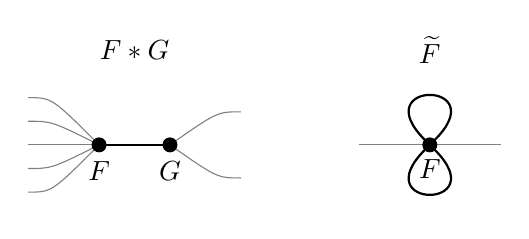
\begin{tikzpicture}[scale=0.6]
    \GraphInit[vstyle=Classic]
    \SetUpEdge[style=-]
    \SetVertexMath
    \tikzset{VertexStyle/.style = {shape=circle, fill=black, minimum size=5pt, inner sep=1pt, draw}}

\def\xsh{7}
    \def\wlen{1.5}

    \foreach \ii in {-2,-1,0,1,2} {
        \draw[thin, color=gray] (-\wlen,\ii*0.5) .. controls +(0.5,0) .. (0,0);
    };

    \foreach \ii in {-1,1} {
        \draw[thin, color=gray] (2*\wlen,\ii*0.7) .. controls +(-0.5,0) .. (\wlen,0);
    };

    \Vertex[x=0,y=0,L=F,Lpos=270]{u}
    \Vertex[x=\wlen,y=0,L=G,Lpos=270]{v}
    \Edge(u)(v)

\draw[thin, color=gray] (\xsh-\wlen, 0) -- (\xsh+\wlen, 0);
    \Vertex[x=\xsh,y=0,L=F,Lpos=270,Ldist=-0.03cm]{w}
    \Loop[dist=1.8cm, dir=NO, style={thick,-}](w)
    \Loop[dist=1.8cm, dir=SO, style={thick,-}](w)

    \node at (\wlen/2,2) {$F * G$};
    \node at (\xsh,2) {$\widetilde{F}$};

\end{tikzpicture}
     \caption{Illustrating (the gadgets with signatures) $F * G$ and $\widetilde{F}$ for 6-ary $F$ and 3-ary $G$.}
    \label{fig:star_tilde}
\end{figure}
See \autoref{fig:star_tilde}.
$F_1 * F_2$ doesn't depend on which inputs we connect, as $F_1$ and $F_2$ are symmetric.
For $\vx \in [q]^{n_1-1}$ and $\vy \in [q]^{n_2-1}$, we have (with vectors viewed as input lists)
\[
    (F_1 * F_2)(\vx,\vy) = \sum_{z \in [q]} F_1(\vx,z) F_2(\vy,z).
\]
\begin{proposition}
    \label{prop:odeco}
    For any $H \in O(q)$, we have
    $HF \in \geneq$ if and only if $H(F * F) \in \geneq$. 
\end{proposition}
\begin{proof}\textcolor{red}{TOPROVE 13}\end{proof}
\begin{theorem}
    \label{thm:odeco}
    Let $\fc$ be a set of real-valued symmetric signatures (tensors). The following are equivalent.
    \begin{enumerate}[label=(\roman*)]
        \item $\fc$ is odeco.
        \item Every connected $\fc$-gadget has a symmetric signature.
        \item For every $F_1,F_2 \in \fc$, $F_1 * F_2$ is symmetric.
    \end{enumerate}
\end{theorem}
Robeva \cite{robeva} conjectured the equivalence of items (i) and (iii) when $\fc$
contains a single signature.
Boralevi, Draisma, Horobeţ, and Robeva \cite{boralevi_orthogonal_2017} confirmed this conjucture
using techniques from algebraic geometry.
We use \autoref{thm:result} to give a combinatorial proof, generalized to arbitrary symmetric
signature sets.
\begin{remark}
    If $\fc$ is a set of symmetric binary signatures, then $F_1 * F_2 = F_1 \circ F_2 = F_1F_2$
    (a matrix product) for $F_1,F_2 \in \fc$. In general, symmetric matrices commute if and only
    if their product is symmetric (as if $F_1F_2$ is symmetric then $F_1F_2 = (F_1F_2)^\top = F_2^\top
    F_1^\top = F_2F_1$ and if $F_1$ and $F_2$ commute then $(F_1F_2)^\top = F_2^\top F_1^\top = F_2F_1 = F_1F_2$).
    Therefore \autoref{thm:odeco} encompasses the extension of the spectral theorem
    which states that commuting symmetric matrices are simultaneously diagonalizable. We use this
    fact in the proof below.
    \label{rem:spectral}
\end{remark}
\begin{proof}\textcolor{red}{TOPROVE 14}\end{proof}
 \section{Possible Variations of \autoref{thm:result}}
\label{sec:variations}
\subsection{Complex-valued signatures}
\label{sec:complex}
Although we have focused on real-valued signatures and matrices, the general and orthogonal 
Holant Theorems hold for complex-valued signatures and matrices. However,
\autoref{thm:result} does not hold for general sets $\fc$ and $\gc$ of complex-valued
signatures, even when we allow $H$ to be complex. For example, Draisma and Regts
\cite{draisma_tensor_2013} consider the \emph{vanishing} unary signature $F \in \rr^{[2]^1}$
defined by $F_0 = 1$ and $F_1 = i$. Any $F$-grid $\Omega$ with at least
one vertex satisfies $\holant_\Omega(F) = 0$, as $\Omega$ is a disjoint union of $K_2$ complete graphs,
with each component having value $f^\top f = [1,i]^\top [1,i] = 0$. 
Thus $F$ is Holant-indistinguishable from 0, but
there is no orthogonal matrix $H$, real or complex, satisfying $Hf = H [1,i]^\top = [0,0]^\top$.

Draisma and Regts also observe that a direct extension of \autoref{thm:duality} to the complex
orthogonal group $O_q(\cc)$ is impossible because $O_q(\cc)$ is not compact. However, they
also provide some techniques for handling complex-valued
signatures in edge coloring models, including a version \cite[Theorem 3]{draisma_tensor_2013} of \autoref{thm:intertwiner_gadget}
for edge-coloring models over any algebraically closed field of characteristic zero.
Cai and Young \cite{cai_planar_2023} and Young \cite{young2022equality} prove their counting
indistinguishability theorems for complex-valued signature sets with the assumption that the sets
are \emph{conjugate-closed}, meaning they must contain the entrywise conjugate of each of their
complex signatures.
It is feasible that \autoref{thm:result} could similarly hold for complex-valued conjugate-closed
$\fc$ and $\gc$ and complex orthogonal $H$ (observe that this invalidates the above counterexample,
as $[1,i]^\top [1,-i] \neq 0$).

\subsection{Quantum orthogonal matrices and planar signature grids}
A \emph{quantum orthogonal matrix} $U$ is, roughly, a matrix whose entries come from an abstract,
not necessarily commutative,
$C^*$-algebra, satisfying the relation $UU^\top = U^\top U = I \otimes \mathbf{1}$, where $\mathbf{1}$
is the identity element of the $C^*$-algebra.
Just as a permutation matrix is an orthogonal matrix that stabilizes $\eq$, 
a \emph{quantum permutation matrix} is a quantum orthogonal matrix that
stabilizes $\eq$ (see e.g. \cite[Equation 27]{cai_planar_2023}). The main theorem of Cai and Young
\cite{cai_planar_2023}, extending the result of Man\v{c}inska and Roberson \cite{planar}, is a planar,
quantum version of \autoref{cor:isomorphism}:
$\fc$ and $\gc$ are $\plholant(\cdot \cup \eq)$-indistinguishabile 
(planar-\#CSP-indistinguishable) if and only if there is a quantum permutation matrix $U$ satisfying
$U \fc = \gc$ ($\fc$ and $\gc$ are \emph{quantum isomorphic}). 
Removing $\eq$, we should obtain the following planar, quantum version of \autoref{thm:result}.
\begin{conjecture}
    \label{con:quantum}
    Let $\fc$, $\gc$ be sets of real-valued signatures. Then the following are equivalent.
    \begin{enumerate}[label=(\roman*)]
        \item $\plholant_{\Omega}(\fc) = \plholant_{\Omega_{\fc\to\gc}}(\gc)$
        for every planar $\fc$-grid $\Omega$.
        \item There is a quantum orthogonal matrix $U$ such that $U\fc = \gc$.
    \end{enumerate}
\end{conjecture}
Cai and Young \cite[Theorem 5]{cai_planar_2023} prove (ii) $\implies$ (i) when $U$ is a quantum permutation matrix;
however, their proof only relies on $U$ being a quantum orthogonal matrix. Therefore,
to prove \autoref{con:quantum}, it suffices to show (i) $\implies$ (ii). The \emph{Tannaka-Krein duality}
for the quantum symmetric group \cite[Theorem 3]{cai_planar_2023} has a more general version
for the quantum orthogonal group $O_q^+$ \cite[Theorem 2.13]{planar}. This version is
analogous to \autoref{thm:duality} above, but concerning quantum subgroups of $O_q^+$ and asymmetric
(planar) tensor categories with duals. Then, following the proof of \cite[Theorem 4]{cai_planar_2023},
but ommitting the gadgets $E^{1,0}$ and $E^{1,2}$ used to construct $\eq$, we will obtain a quantum analogue
of our \autoref{thm:intertwiner_gadget} for planar quantum $\fc$-gadgets, giving a quantum
analogue of \autoref{lem:offdiagblock}. The rest of the proof of \autoref{thm:result}, however, involves
nonplanar signature grid manipulations (e.g. in \autoref{fig:grid_trace} it is in general impossible to embed $\Omega$ such that 
every instance of $D$ lies on the outer face) and, more critically, relies on the existence of the
singular value decomposition of a submatrix of a real orthogonal matrix, then on viewing the resulting
diagonal matrix as a signature. It is yet unclear whether the same or similar reasoning applies to a
submatrix of a quantum orthogonal matrix.
 
\subsection*{Acknowledgements}
The author thanks Jin-Yi Cai for helpful discussions and Ashwin Maran for his suggestion which
improved the proof of \autoref{thm:odeco}. The author also thanks Guus Regts for pointing out
reference \cite{schrijver_graph_2008}.

\appendix
\section{Block Signature Actions}
\label{sec:appendix_block}
In this appendix, we prove several technical results which state that the action of a 
block matrix $H$ on a block signature $K$ follows block matrix multiplication rules as one would expect.
\begin{proposition}
    \label{prop:block}
    Let $\ic = X \sqcup Y$.
    For $H \in \rr^{\ic\times\ic}$, $K^{m,d} \in \rr^{\ic^m \times \ic^d}$ and any $\vr\in\{X,Y\}^m$
    $\vc\in\{X,Y\}^d$,
    \[
        (H^{\otimes m} K^{m,d})|_{\vr,\vc} = 
        \sum_{\vj \in \{X,Y\}^m} \left(\bigotimes_{i=1}^m H|_{R_i,J_i}\right) K^{m,d}|_{\vj,\vc}
    \]
    (with $H^{\otimes m} K^{m,d} \in \rr^{\ic^m \times \ic^d}$ 
    indexed as in part 3 of \autoref{def:block}) and similarly
    \[
        (K^{m,d}H^{\otimes d})|_{\vr,\vc} = 
        \sum_{\vj \in \{X,Y\}^d}  K^{m,d}|_{\vr,\vj}\left(\bigotimes_{i=1}^d H|_{J_i,C_i}\right).
    \]
\end{proposition}
That is, with $H^{\otimes m}|_{\vr,\vj} = \bigotimes_{i=1}^m H|_{R_i,J_i}$,
we can compute $H^{\otimes m}K^{m,d}$ as a block matrix product with
\[
    H^{\otimes m} = 
    \begin{bmatrix} 
        H^{\otimes m}|_{X^{m},X^{m}} &
        H^{\otimes m}|_{X^{m},X^{m-1}Y} & 
        H^{\otimes m}|_{X^{m},X^{m-2}YX} & \ldots & 
        H^{\otimes m}|_{X^{m},Y^{m}}\\
        H^{\otimes m}|_{X^{m-1}Y,X^{m}} &
        H^{\otimes m}|_{X^{m-1}Y,X^{m-1}Y} & 
        H^{\otimes m}|_{X^{m-1}Y,X^{m-2}YX} & \ldots & 
        H^{\otimes m}|_{X^{m-1}Y,Y^{m}}\\
        \vdots & \vdots & \vdots && \vdots \\
        H^{\otimes m}|_{Y^{m-1}X,X^{m}} & 
        H^{\otimes m}|_{Y^{m-1}X,X^{m-1}Y} &
        H^{\otimes m}|_{Y^{m-1}X,X^{m-2}YX} & \ldots & 
        H^{\otimes m}|_{Y^{m-1}X,Y^{m}}
        \\
        H^{\otimes m}|_{Y^{m},X^{m}} 
        & H^{\otimes m}|_{Y^{m},X^{m-1}Y} 
        & H^{\otimes m}|_{Y^{m},X^{m-2}YX} 
        & \ldots & H^{\otimes m}|_{Y^{m},Y^{m}} 
    \end{bmatrix}
\]
and
\[
    K^{m,d} =
    \begin{bmatrix} 
        K^{m,d}|_{X^{m},X^{d}} &
        K^{m,d}|_{X^{m},X^{d-1}Y} & \ldots &
        K^{m,d}|_{X^{m},Y^{d-1}X} & 
        K^{m,d}|_{X^{m},Y^{d}}\\
        K^{m,d}|_{X^{m-1}Y,X^{d}} &
        K^{m,d}|_{X^{m-1}Y,X^{d-1}Y} & \ldots & 
        K^{m,d}|_{X^{m-1}Y,Y^{d-1}X} & 
        K^{m,d}|_{X^{m-1}Y,Y^{d}}\\
        K^{m,d}|_{X^{m-2}YX,X^{d}} & 
        K^{m,d}|_{X^{m-2}YX,X^{d-1}Y} &\ldots & 
        K^{m,d}|_{X^{m-2}YX,Y^{d-1}X} & 
        K^{m,d}|_{X^{m-2}YX,Y^{d}} \\
        \vdots & \vdots && \vdots & \vdots \\
        K^{m,d}|_{Y^{m},X^{d}} &
        K^{m,d}|_{Y^{m},X^{d-1}Y} & \ldots & 
        K^{m,d}|_{Y^{m},Y^{d-1}X} &
        K^{m,d}|_{Y^{m},Y^{d}}.
    \end{bmatrix}.
\]
\begin{proof}\textcolor{red}{TOPROVE 15}\end{proof}
We will only need \autoref{prop:block} as written, for partitions of $\ic$ into two blocks, but it is
not hard to see that it extends naturally to partitions of $\ic$ into more than two blocks.

We will apply \autoref{prop:block} for two special types of $H$.
\begin{corollary}
    \label{cor:on_diag_block}
    If 
    \[
        H = H_X \oplus H_Y = \begin{bmatrix} H_X & 0 \\ 0 & H_Y\end{bmatrix}
    \]
    is block-diagonal, then, for any $K \in \rr^{\ic^n}$, 
    the block form of $H^{\otimes n} K^{n,0}$ is
    \[
        \begin{bmatrix} 
            H_X^{\otimes n} & 0 & \ldots & 0 & 0\\
            0 & * & \ldots & 0 & 0\\
            \vdots & \vdots & \ddots & \vdots & \vdots \\
            0 & 0 & \ldots & * & 0\\
            0 & 0 & \ldots & 0 & H_Y^{\otimes n}
        \end{bmatrix}
        \begin{bmatrix} 
            (K|_X)^{n,0} \\ * \\ \vdots \\ * \\ (K|_Y)^{n,0}
        \end{bmatrix} =
        \begin{bmatrix} 
            H_X^{\otimes n}(K|_X)^{n,0} \\ * \\ \vdots \\ * \\ H_Y^{\otimes n}(K|_Y)^{n,0}
        \end{bmatrix}.
    \]
\end{corollary}
\begin{proof}\textcolor{red}{TOPROVE 16}\end{proof}
If $X = V(F)$, $Y = V(G)$, and $K = F \oplus G$, then by \eqref{eq:oplus_index},
all blocks of $K$ are 0 except $K|_X = F$ and $K|_Y = G$, so, by \autoref{cor:on_diag_block},
\begin{equation}
    \label{eq:oplus_action}
    (H_{V(F)} \oplus H_{V(G)})(F \oplus G) = (H_{V(F)} F) \oplus (H_{V(G)} G).
\end{equation}

\begin{corollary}
\label{cor:off_diag_block}
If
\[
    B = \begin{bmatrix} 0 & H^\top \\ H & 0 \end{bmatrix}
\]
is block-antidiagonal, with blocks indexed by $X = V(F)$ and $Y = V(G)$, then, for any $m,d$,
\[
    H^{\otimes m}F^{m,d} = G^{m,d}H^{\otimes d} \text{~~and~~}
    (H^\top)^{\otimes m}G^{m,d} = F^{m,d}(H^\top)^{\otimes d}
    \iff 
    B^{\otimes m}(F \oplus G)^{m,d} = (F \oplus G)^{m,d}B^{\otimes d}.
\]
\end{corollary}
\begin{proof}\textcolor{red}{TOPROVE 17}\end{proof}
 
\printbibliography

\end{document}
